\documentclass[a4paper, 13pt]{report}
\usepackage{comment} % enables the use of multi-line comments (\ifx \fi) 
\usepackage{lipsum} %This package just generates Lorem Ipsum filler text. 
\usepackage{fullpage} % changes the margin
\usepackage[utf8]{vietnam}
\usepackage{amsmath}
\usepackage{graphicx}
\graphicspath{ {images/} }
\usepackage{caption}
\usepackage{enumitem}
\usepackage{array}
\newcommand\tab[1][1cm]{\hspace*{#1}}
\newenvironment{steps}[1]{\begin{enumerate}[label=#1 \arabic*]}{\end{enumerate}}
\usepackage{placeins}
\usepackage{pbox}
\newcommand\SLASH{\char`\\}
\usepackage{fancybox}
\usepackage{placeins}
\usepackage[document]{ragged2e}
\usepackage{relsize}
\usepackage{amssymb}
\usepackage{ctable} % for \specialrule command
\usepackage{multirow}
\usepackage{wrapfig}
\usepackage{subcaption}
\setcounter{tocdepth}{1} % for \tableofcontents



\makeatletter% http://tex.stackexchange.com/questions/29517/forcing-new-line-after-item-number-in-enumerate-environment/29518#29518
\def\step{%
   \@ifnextchar[ \@step{\@noitemargtrue\@step[\@itemlabel]}}
\def\@step[#1]{\item[#1]\mbox{}}
\makeatother

\begin{document}

\newpage
\pagenumbering{gobble}  % ------- bỏ đánh số trang----------------
% trang bìa 1-----------------------------------------------------
	%\thispagestyle{empty}
	\thisfancypage{
		\doublebox}
	{}
	
	\begin{center}
		\vspace*{0.2cm}
		ĐẠI HỌC QUỐC GIA TP. HỒ CHÍ MINH\\
		{\fontsize{14pt}{1}\textbf{		TRƯỜNG ĐẠI HỌC BÁCH KHOA }}\\
		-------------------------------\\
		
\includegraphics[width=3cm]{images/bk}\\
		\vspace*{2cm}
		{\fontsize{14pt}{1}\selectfont LÊ THỊ MINH THÙY}\\
		\vspace*{2cm}
		{\fontsize{16pt}{1}\selectfont \textbf{DỰ ĐOÁN XÁC SUẤT \\ THỜI GIAN XE BUÝT VỀ ĐÚNG TRẠM}}\\
		\vspace*{2cm}
		\begin{flushleft}
		\large
		\begin{tabular}{ ll } 
        \hspace{1cm} Chuyên ngành: & Khoa học máy tính\\
		\hspace{1cm} Mã số: & 60.48.01\\
		\end{tabular}
		\end{flushleft}
		\vspace*{2cm}
		{\fontsize{14pt}{1}\selectfont LUẬN VĂN THẠC SĨ}\\
		\vspace*{2cm}
		{\fontsize{12pt}{1}	TP.Hồ Chí Minh, \today}\\
		\vspace*{2cm}
		{\fontsize{12pt}{1}	Công trình được hoàn thành tại:\\ Trường Đại Học Bách Khoa - ĐHQG - TPHCM}
	\end{center}
%----------------------------------------------------------------------------------------	
\pagebreak
Công trình được hoàn thành tại: \textbf{Trường Đại Học Bách Khoa - ĐHQG - TPHCM}\\
Cán bộ hướng dẫn khoa học: TS. Huỳnh Tường Nguyên	\\
	(Ghi rõ họ, tên, học hàm, học vị và chữ  ký)\\

\vspace*{4cm}Cán bộ chấm nhận xét 1: 	\\
	(Ghi rõ họ, tên, học hàm, học vị và chữ  ký)\\

\vspace*{4cm}Cán bộ chấm nhận xét 2:	\\
	(Ghi rõ họ, tên, học hàm, học vị và chữ  ký)\\

\vspace*{4cm}Luận văn thạc sĩ được bảo vệ tại Trường Đại học Bách Khoa, ĐHQG Tp. HCM \\
\today.

\vspace*{0.5cm}Thành phần đánh giá hội đồng luận văn thạc sĩ bao gồm: \\
1.  (Chủ tịch)\\
2.  (Thư ký)	\\
3.  (Phản biện 1)\\
4.  (Phản biện 2)\\
5.  (Uỷ viên)\\
Xác nhận của Chủ tịch Hội đồng đánh giá luận văn và Trưởng khoa quản lý chuyên ngành sau khi luận văn đã được sửa chữa (nếu có).\\
\begin{tabular}{ p{7cm}p{9cm}}
 \hspace{1cm} CHỦ TỊCH HỘI ĐỒNG & TRƯỞNG KHOA KH$\&$KT Máy Tính\\
 \hspace{1cm}  (Họ tên và chữ ký) & (Họ tên và chữ ký)\\
\end{tabular}\\
\pagebreak
%----------------------------------------------------------------------------------------
\begin{tabular}{ p{7cm}p{9cm}}
 ĐẠI HỌC QUỐC GIA TP. HỒ CHÍ MINH & \textbf{CỘNG HÒA XÃ HỘI CHỦ NGHĨA VIỆT NAM}\\
 \hspace{0.5cm}TRƯỜNG ĐẠI HỌC BÁCH KHOA & \hspace{2cm}\textbf{Độc lập - Tự do - Hạnh phúc}\\
\end{tabular}\\
\vspace*{1cm}
\begin{center}{\fontsize{16pt}{1}\selectfont \textbf{NHIỆM VỤ LUẬN VĂN THẠC SĨ}}\\\end{center}
\begin{tabular}{ ll}
\vspace*{0.1cm}Họ tên học viên: Lê Thị Minh Thùy&\vspace*{0.1cm} MSHV: 13070269\\
\vspace*{0.1cm} Ngày, tháng, năm sinh: 22/01/1986 &\vspace*{0.1cm} Nơi sinh: Đồng Nai\\
\vspace*{0.1cm} Ngành: Khoa học máy tính & \vspace*{0.1cm} Mã số: 60.48.01\\
\multicolumn{2}{l}{\vspace*{1cm}I. TÊN ĐỀ TÀI: Dự đoán xác suất thời gian xe buýt về trạm đúng giờ} \\
\vspace*{0.1cm} II.  NHIỆM VỤ VÀ NỘI DUNG: \\
\multicolumn{2}{l}{\vspace*{0.1cm}1. Tìm thuật toán đơn giản, phù hợp để giải bài toán} \\
\multicolumn{2}{l}{\vspace*{3cm}2. Hiện thực để chứng minh thuật toán đã chọn lập trình được} \\

\vspace*{0.1cm} III.  NGÀY GIAO NHIỆM VỤ: & \\
\vspace*{0.1cm} IV.  NGÀY HOÀN THÀNH NHIỆM VỤ: & \\
\vspace*{0.1cm}V. CÁN BỘ HƯỚNG DẪN: TS. Huỳnh Tường Nguyên & \\
\end{tabular}\\
\vspace*{1cm}
\hfill Tp. HCM, \today. 
\begin{tabular}{ p{7cm}p{9cm}}
 \hspace{1cm} CÁN BỘ HƯỚNG DẪN & TRƯỞNG KHOA KH$\&$KT Máy Tính\\
 \hspace{1cm}  (Họ tên và chữ ký) & (Họ tên và chữ ký)\\
\end{tabular}\\
%----------------------------------------------------------------------------------------
\pagebreak
\begin{center}{\fontsize{16pt}{1}\selectfont \textbf{LỜI NÓI ĐẦU}}\\\end{center}
Để hoàn thành được Luận Văn Thạc Sĩ ngày hôm nay, tôi chân thành cảm ơn 4 năm được học tập chương trình Thạc Sĩ Khoa Học Máy Tính tại trường Đại Học Bách Khoa cùng với sự giảng dạy tận tình của thầy cô và cơ hội trao đổi kinh nghiệm quý báu với các bạn cùng khóa.\\
Trong chương Cơ sở lý thuyết của Luận Văn Thạc Sĩ của mình, tôi có sao chép một phần nội dung trong sách dịch tiếng Việt tên là "Thống kê Công nghiệp hiện đại với ứng dụng viết trên R, MINITAB và JMP", bản quyền tiếng Việt của Viện Nghiên cứu cao cấp về Toán. Tôi xin phép không trả tiền bản quyền sử dụng, do Luận Văn Thạc Sĩ của mình chỉ sử dụng chúng như là bằng chứng kham khảo cho ngày bảo vệ hội đồng Thạc Sĩ, không dùng mục đích thương mại hay bất kỳ hoạt động khoa học nào, nghĩa là, tôi cam đoan không đem nội dung Luận Văn này để mua bán, đăng báo hay thuyết trình bất cứ đâu.\\
Đồng thời, tôi khuyến cáo người đọc nên tiếp cận nội dung lý thuyết phiên bản tiếng Anh.
\begin{flushright}
\today\\
Lê Thị Minh Thùy
\end{flushright}
%-----------------------------------------------------------------------------------------
\pagebreak
\begin{center}{\fontsize{16pt}{1}\selectfont \textbf{TÓM TẮT LUẬN VĂN}}\\\end{center}
%-----------------------------------------------------------------------------------------
\pagebreak
\begin{center}{\fontsize{16pt}{1}\selectfont \textbf{ABSTRACT}}\\\end{center}
%-------------------------------------------------------------------------------------------
\pagebreak
\begin{center}{\fontsize{16pt}{1}\selectfont \textbf{LỜI CAM ĐOAN}}\\\end{center}
Tôi cam đoan rằng, ngoại trừ các kết quả tham khảo từ các công trình khác như đã ghi rõ trong luận văn, các công việc trình bày trong luận văn này do chính tôi thực hiện và không nội dung nào của luận văn này đã được nộp để lấy một bằng cấp ở trường này hoặc trường khác.\\
\begin{flushright}
\today\\
Lê Thị Minh Thùy
\end{flushright}
\iffalse
%comment
\fi
\tableofcontents
\pagebreak
\pagenumbering{arabic}
\chapter{GIỚI THIỆU ĐỀ TÀI} %%%%%%%%%%%%%%%%%%%%%%%%%%%%%%%%
\section{Giới thiệu đề tài}
Theo nghiệp vụ xe buýt, các bác tài xế chỉ có khoảng thời gian cố định cộng thêm linh động trễ thêm vài phút để hoàn tất một lộ trình đã vạch sẵn. Khi lái xe lâu năm trên một lộ trình giống nhau, các bác tài xế khi đi được một phần đoạn đường, họ sẽ ước lượng quãng thời gian còn lại có hoàn thành kịp tiến độ cho quãng đường còn lại hay không. Mục đích Luận Văn: dùng Toán định lượng kinh nghiệm nhắm chừng này.\\
Có dữ liệu di chuyển 2/3 chặng đi từ BX Củ Chi - BX An Sương của tuyến xe buýt 74 và kết quả tương ứng về trạm đích: đúng giờ hay trễ giờ. Sử dụng thao tác khai phá dữ liệu học có quan sát, phân chia dữ liệu thành 2 phần: phần để học có kèm theo kết quả về trạm đích, phần để kiểm tra đã loại bỏ nhãn đúng giờ hay trễ giờ tại trạm đích.\\
Do quan sát kích thước mẫu giới hạn, ngẫu nhiên các chuyến di chuyển từ BX Củ Chi - BX An Sương (tuyến xe buýt 74 ngẫu nhiên được chọn) kèm theo kết quả về trạm đích đúng giờ hay trễ giờ tương ứng. Vì kích thước mẫu giới hạn, không sử dụng sức mạnh tính toán hiệu năng cao trên kích thước dữ liệu siêu lớn, Luận Văn dùng kiến thức Thống Kê, làm việc trên kích thước mẫu chấp nhận được so với trên tổng thể quá to lớn nhưng  đủ rút ra đặc trưng cho tổng thể để giải quyết bài toán trên.\\
Ngoài ra, Luận Văn dùng kiến thức xác suất, con số đo khả năng một sự kiện xảy ra vì ta chấp nhận dự đoán dựa trên 2/3 chặng đường ban đầu, trong khi đó 1/3 chặng đường sau vẫn có tác động đến kết quả dự đoán. Khi dùng xác suất, ta chấp nhận bài toán có sự tham gia không chắc chắn, có thay đổi do ngẫu nhiên.\\
Trên thực tế rất hiếm hai chuyến xe cùng lộ trình có những bước di chuyển cách nhau 20 giây giống nhau hoàn toàn, do đó Luận Văn dùng ước lượng tham số trong kiến thức Thống Kê để mô hình hóa di chuyển.\\  
Công thức xác suất Bayes $\mathbb{P}(B|A) = \frac{\mathbb{P}(B) \cdot \mathbb{P}(A|B)}{\mathbb{P}(A)}$ phù hợp để giải bài toán dán nhãn dự đoán về trạm đích đúng giờ hay trễ giờ (biến cố B) cho di chuyển 2/3 chặng của tuyến đi cố định từ BX Củ Chi - BX An Sương (biến cố A), vì khi ta quan sát biến cố A xảy ra và có xác suất có điều kiện $\mathbb{P}(A|B)$ được biết trước, lý thuyết Bayes cho ta cách tính để đánh giá xác suất một sự kiện B chưa quan sát được xảy ra sau khi biến cố A đã xảy ra.\\
Tổng kết lại, mục đích Luận Văn: dùng kiến thức Thống kê, xác suất, công thức xác suất Bayes để mô hình dữ liệu học, dùng mô hình này để dán nhãn đúng giờ hay trễ giờ cho dữ liệu kiểm tra.\\

\section{Động cơ}
Hiện nay, có nhiều ứng dụng hay nghiên cứu khoa học khai thác thông tin GPS của các chuyến xe buýt di chuyển trên địa bàn TP. Hồ Chí Minh để rút trích thông tin có ích với mong muốn với tri thức mới tìm được trong dữ liệu thô có thể giúp ích và cải thiện dịch vụ phục vụ của phương tiện giao thông công cộng này.\\
\section{Mục tiêu}
Luận Văn bó hẹp với đề bài cụ thể: Dùng Toán Thống Kê định lượng kinh nghiệm di chuyển trên cùng một lộ trình để dán nhãn về trạm đúng giờ hay trễ giờ.\\
Luận Văn không đặt mục tiêu tham vọng giải bài toán này có thể đem ra ứng dụng thực tế được vì bản thân người giải bài toán không có nhiều kinh nghiệm với Toán Thống Kê, làm việc với kích thước mẫu rất nhỏ có thể đưa ra dự đoán đúng trên kích thước quần thể.\\
Ngoài ra, người lái xe phải hiểu rằng kết quả dự đoán về trạm đích đúng giờ chỉ mang tính xác suất. Ví dụ, sau khi đi được 2/3 chặng, bác tài xế nhận được kết quả xác suất 98.5\% xe về trạm đúng giờ. Nhưng gặp sự cố tại 1/3 chặng đường cuối, tình trạng kẹt xe nặng, xe về trạm không đúng giờ như kết quả thông báo trên với con số xác suất đúng giờ xảy ra rất lớn 98.5\%. Bác tài xế phải chấp nhận xác suất 1.5\% về trạm trễ giờ vẫn có khả năng xảy ra do bác tài xế không thể điều khiển tình trạng xe chạy tại 1/3 chặng đường cuối. Nhưng các con số xác suất được thông báo cho bác tài vẫn có ý nghĩa chừng mực nếu bác tài xế biết rằng các con số xác suất này định lượng kinh nghiệm những chuyến di chuyển trong quá khứ để dự báo tương lai cho chuyến đi hiện tại. Khi đã hiểu được định nghĩa xác suất, hiểu được các sự kiện xảy ra trên thực tế không bao giờ được dự đoán chắc chắn 100\% xảy ra, mà chỉ dự đoán khả năng có thể xảy ra, người đọc chấp nhận bài toán được giải trong Luận Văn này phần nào có ý nghĩa.\\
Tóm lại, tác giả nhắc lại mục tiêu rất cụ thể của Luận Văn này: Dùng Toán Thống Kê định lượng kinh nghiệm di chuyển trên cùng một lộ trình để dán nhãn về trạm đúng giờ hay trễ giờ.
\section{Phương pháp nghiên cứu}
Phương pháp nghiên cứu là thu thập dữ liệu di chuyển hữu hạn, quan sát các bước di chuyển được ghi nhận cách nhau 20 giây trên 2/3 lộ trình đi từ BX Củ Chi - BX An Sương, trực quan hóa dữ liệu này, cộng thêm kiến thức quan sát thực tế, nếu có nhiều bước di chuyển dài trong từng khoảng 20 giây thì chuyến đi đó có khả năng về trạm đúng giờ cộng thêm kết quả dán nhãn về trạm đúng giờ hay trễ giờ chỉ cho ta biết khả năng xảy ra, chứ không phải chắc chắn. Những kiến thức này giúp ta nghĩ đến kiến thức Thống Kê, xác suất chủ đạo và từ đó từng bước tìm thuật toán, công thức phù hợp để giải. Tóm lại, nhờ quan sát dữ liệu cho ta định hướng cách tiếp cận, cách nghiên cứu.  
\section{Một số kết quả thu được}
\section{Cấu trúc luận văn}
\pagebreak
\chapter{CƠ SỞ LÝ THUYẾT}
\section{Lý thuyết xác suất cơ bản}
\subsection*{Tổng thể và mẫu}
Kham khảo trang 19, 24, 25 chương 2 từ sách \cite{TKCNUDR}
\begin{itemize}
\item Một \textbf{tổng thể} (còn được gọi là quần thể) thống kê là một tập các phần tử có một thuộc tính chung nhất định. 
\\Ví dụ, tập hợp tất cả các chuyến xe buýt từ BX Củ Chi - BX An Sương của tuyến 74 vào ngày 17 tháng 10 năm 2016 là một tổng thể hữu hạn và có thực.\\
Một ví dụ khác, tập tất cả các chuyến xe buýt từ BX Củ Chi - BX An Sương của tuyến 74 có thể về trạm trễ trong điều kiện: mưa nhiều, đường ngập, hẹp, rào chắn lô cốt, quá tải xe máy xuyên suốt cả ngày và va chạm xe máy thường xuyên. Tổng thể này là vô hạn và giả định.
\item Một \textbf{mẫu} là một tập hợp các phần tử trong một tổng thể nhất định. Một mẫu thường được chọn ra từ một tổng thể với mục tiêu quan sát các đặc tính của tổng thể ấy và đưa ra các quyết định thống kê có liên quan đến các đặc trưng tương ứng. \\
Chẳng hạn, xét vài trăm triệu chuyến xe từ BX Củ Chi - BX An Sương của tuyến 74, công ty quản lý muốn tìm ra được đặc trưng tình trạng di chuyển 2/3 chặng đường như thế nào để cảnh báo sớm tình trạng đến đích trễ cho các bác tài xế. Nếu không sử dụng sức mạnh tính toán của điện toán đám mây, chỉ có giới hạn sức tính toán của con người, những nhà thống kê sẽ rút ra đặc trưng của vài trăm triệu dữ liệu bằng cách làm việc trên mẫu ngẫu nhiên rút ra từ vài trăm triệu dữ liệu trên. Những thủ tục lấy mẫu như vậy để đưa ra các quyết định thống kê được gọi là phương pháp lấy mẫu chấp nhận. Ngoài ra, Toán Thống Kê cung cấp phương pháp ước lượng bằng cách sử dụng các mẫu chọn ra từ các tổng thể hữu hạn, bao gồm cả việc lấy mẫu ngẫu nhiên có hoàn lại và lấy mẫu ngẫu nhiên không hoàn lại.\\
\end{itemize}
Như vậy, trong Toán Thống Kê, tồn tại các phương pháp như phương pháp thí nghiệm thống kê, phương pháp lấy mẫu chấp nhận, phương pháp kiểm định giả thuyết,.. để từ mẫu ngẫu nhiên đủ rút ra đặc trưng của tổng thể với xác suất xảy ra cao. Nhưng để thực hiện được điều này, nó vượt quá kiến thức kỹ sư máy tính. Cho nên Luận Văn này không đặt tham vọng, giải trên mẫu có thể kết luận trên tổng thể với xác suất xảy ra cao.\\
Ngoài ra, tôi có đưa thêm một số giả định trong khi xem xét mẫu được lấy ngẫu nhiên trong Luận Văn: 
\begin{itemize}
\item Tôi tập trung vào đo lường chuyến đi trong một khoảng thời gian cụ thể, tháng 9 năm 2016, các mẫu của tôi không rải rác qua các tháng, các năm. 
\item  Chúng ta chỉ dự đoán được một phần trong nhiều hiện tượng mà ta gặp phải. Xem xét tất cả các chuyến xe trên mọi điều kiện không thể kiểm soát được trên thực tế là quá tốn kém và không thực tế. Cho nên các yếu tố bên ngoài như thời điểm xuất phát, thời tiết, điều kiện mặt đường,... được coi là các yếu tố độc lập để giảm sự phức tạp giải bài toán.
\end{itemize}  
\subsection*{Biến cố và không gian mẫu: Diễn tả hình thức của thí nghiệm}
Kham khảo trang 52, 55, 59, 60, 61, 63 chương 3 từ sách \cite{TKCNUDR}
Ta thấy cùng một tuyến đường xe buýt 74 cố định, từ BX Củ Chi - BX An Sương, các chuyến xe trong cùng tháng 9 có thời gian hoàn thành khác nhau, không biết trước được một cách chắc chắn. Nguyên nhân là do những yếu tố bên ngoài như mặt đường, thời tiết, giờ cao điểm, thấp điểm,..đều có ảnh hưởng đến kết quả. Toán Thống Kê giúp ta có phương pháp làm việc trên dữ liệu có tính ngẫu nhiên như vậy.\\
\textbf{Không gian mẫu} là tập hợp của tất cả các kết cục có thể của một thí nghiệm cụ thể. Chẳng hạn, thí nghiệm tung một đồng xu, kết quả ngẫu nhiên là ngửa (Head, $\mathcal{H}$) hoặc sấp (Tail, $\mathcal{T}$), cho ta không gian mẫu $\mathcal{S= \{H,T}\}$. Các \textbf{biến cố sơ cấp} hay \textbf{điểm mẫu} là những phần tử của $\mathcal{S}$.\\
\subsection*{Xác suất của biến cố}
Thông thường chúng ta gộp tất cả các biến cố vào một tập $\mathcal{Q}$ := $\{ A: A \subset \mathcal{S}$ là một biến cố$\}$, gọi là tập các biến cố.\\
Xét một hàm $\mathbb{P}: \mathcal{Q} \rightarrow \mathbb{R}$ xác định trên $\mathcal{Q}$, gán cho mỗi biến cố A một số thực, ký hiệu A $\mapsto$ $\mathbb{P}$[A], $\mathbb{P}$[A] (hay $\mathbb{P}$(A)) là khả năng hoặc cơ hội mà biến cố A xảy ra. $\mathbb{P}$ được gọi là hàm xác suất khi thỏa mãn những tiên đề cơ bản sau đây:\\
\begin{itemize}
\item $\textbf{A1}$ Xác suất là không âm, $\mathbb{P}$(A) $\geq$ 0
\item $\textbf{A2}$ Không gian mẫu $\mathcal{S}$ có xác suất 1, $\mathbb{P}(\mathcal{S})$=1
\item $\textbf{A3}$ Xác suất của các biến cố rời nhau. Khi có hai biến cố A, B mà A $\cap$ B = $\emptyset$ thì\\
\begin{center}
$ \mathbb{P}(A \cup B) = \mathbb{P}(A $ hay $B) = \mathbb{P}(A) + \mathbb{P}(B)$
\end{center}
Tổng quát hơn, nếu ta có $E_{1}, E_{2},...,E_{n}$ (n $\geq$ 1) là các biến cố rời nhau từng đôi một thì\\
\[
\mathbb{P}\left[\bigcup_{i=1}^n E_{i}\right]=\sum_{i=1}^n \mathbb{P}[E_i]
\]
\end{itemize}
\subsection*{Xác suất có điều kiện và sự độc lập của các biến cố}
Khi các biến cố khác nhau có liên quan, việc thực hiện một biến cố có thể cung cấp cho ta thông tin liên quan để cải thiện, nâng cao khả năng đánh giá của ta về các biến cố khác. Biến cố B đã xảy ra, tức là $\mathbb{P}[B]$ > 0, xác suất biến cố A cũng xảy ra là gì? Suy nghĩ một cách tích cực, ta thấy nên thu hẹp không gian mẫu S tới không gian trong đó B đã xảy ra (nhằm mục đích so sánh giữa A $\cap$ B và B)
\textbf{Xác suất có điều kiện} của biến cố A cho biết biến cố B đã xảy ra, $\mathbb{P}[B]$ > 0 là
\[
\mathbb{P}(A|B)=\frac{\mathbb{P}(AB)}{\mathbb{P}(B)}=\frac{\mathbb{P}(A\cap B)}{\mathbb{P}(B)}
\]
Theo đó xác suất đồng thời của hai biến cố A và B là
\[
\mathbb{P}(AB)=\mathbb{P}(A\cap B)=\mathbb{P}(B)\cdot \mathbb{P}(A|B)
\]
Ví dụ: Thí nghiệm đo chiều dài của một thanh thép. Không gian mẫu là $\mathcal{S}$ = (19.5, 20.5)[cm]. Hàm xác suất gán bất kỳ một khoảng tập con của S một xác suất bằng chiều dài của nó. Cho A = (19.5,20.1), nghĩa là $\mathcal{P}(A)$ = 20.1-19.6=0.6 và B = (19.8,20.5), nghĩa là $\mathcal{P}(B)$ = 20.5-19.8=0.7. Khoảng tập con chung giữa A$\cap$B=(19.8,20.1), nghĩa là $\mathcal{P}(A\cap B)$ = 20.1-19.8=0.3.\\
Cho một độ dài và biết thêm điều kiện độ dài này thuộc khoảng B, và chúng ta phải đoán xem nó có thuộc về A không? Ta tính xác suất có điều kiện
\[
\mathbb{P}(A|B)=\frac{\mathbb{P}(AB)}{\mathbb{P}(B)}=\frac{\mathbb{P}(A\cap B)}{\mathbb{P}(B)}=\frac{0.3}{0.7}=0.4286
\]
Mặt khác, nếu thông tin độ dài thuộc về B không biết trước, thì với độ dài của câu hỏi trên, xác suất nó thuộc về A bằng $\mathbb{P}(A)$=0.6. Vậy có một sự khác biệt giữa xác suất có điều kiện và không điều kiện. Điểu này cho thấy hai biến cố A và B là phụ thuộc.\\
Hai biến cố A và B được gọi là \textbf{độc lập} nếu
\[
\mathbb{P}(A|B)=\mathbb{P}(A)
\]
Nói khác đi, biến cố A và B độc lập nếu sự xuất hiện của A không có liên quan theo bất kỳ cách nào đến sự xuất hiện của B: $\mathbb{P}(A|B)=\mathbb{P}(A)$ và $\mathbb{P}(B|A)=\mathbb{P}(B)$\\
Nếu A và B là các biến cố độc lập thì 
\[
\mathbb{P}(A)=\mathbb{P}(A|B)=\frac{\mathbb{P}(A\cap B)}{\mathbb{P}(B)}
\]
hay tương đương với 
\[
\mathbb{P}(AB)=\mathbb{P}(A\cap B)=\mathbb{P}(A)\cdot\mathbb{P}(B_j)
\]
nghĩa là xác suất hai biến cố độc lâp đồng thời xảy ra bằng tích các xác suất riêng lẻ.\\
Tổng quát, các biến cố $A_{1}, A_{2},..., A_{n}$ là n biến cố \textbf{độc lập lẫn nhau} thì
\[
\mathbb{P}\left[\bigcap_{i=1}^n A_j \right] = \prod_{i=1}^n \mathbb{P}[A_i]
\]

\subsection*{Công thức Bayes và ứng dụng của nó}
Công thức Bayes cho ta cách thức cơ bản để đánh giá bằng chứng trong các dữ liệu liên quan đến các thông số chưa biết, hoặc một số biến cố không quan sát được. Giả sử rằng một thí nghiệm ngẫu nhiên cho kết quả trong một biến cố A (hoặc phần bù của nó), ngoài ra các kết quả này phụ thuộc vào một biến cố B mà ta không trực tiếp quan sát được, nhưng xác suất có điều kiện $\mathbb{P}$(A|B) là được biết trước.\\
Bayes nói biến cố quan sát được A có liên quan đến biến cố B không quan sát được thông qua các xác suất có điều kiện. Để cân nhắc bằng chứng cho thấy A có ảnh hưởng trên B, diễn đạt bởi $\mathbb{P}(B|A)$ đầu tiên chúng ta giả định một xác suất $\mathbb{P}$(B) mà được gọi là xác suất tiên nghiệm. Xác suất tiên nghiệm $\mathbb{P}(B)$ thể hiện mức độ tin tưởng của chúng ta vào sự xảy ra của biến cố B. Ta luôn có điều kiện sau, cho phép tính xác suất hậu nghiệm $\mathbb{P}(B|A)$, là xác suất B xảy ra sau khi quan sát A (nên có mẫu số $\mathbb{P}$(A))\\
\[
\mathbb{P}(B|A) = \frac{\mathbb{P}(B) \cdot \mathbb{P}(A|B)}{\mathbb{P}(A)}
\]
Tổng quát, giả sử $\{$B$_1$,...,B$_m\}$ là một phân vùng của không gian mẫu. Các biến cố B$_1$,...,B$_m$ không trực tiếp quan sát hay kiểm chứng được, nhưng các xác suất có điều kiện $\mathbb{P}(A|B_i)$ là được biết trước. Giả định các xác suất tiên nghiêm là $\mathbb{P}(B_i)$, thể hiện mức độ tin tưởng của ta vào sự xảy ra của biến cố B$_i$. Sau khi quan sát A ta chuyển đổi các xác suất tiên nghiệm của B$_{i}$ thành các xác suất hậu nghiệm $\mathbb{P}(B_i|A)$, theo trên\\
\[
\mathbb{P}(B_i|A) = \frac{\mathbb{P}(B_i) \cdot \mathbb{P}(A|B_i)}{\mathbb{P}(A)}
\]
Vì $\{$B$_1$,...,B$_m\}$là một phân vùng 	của $\mathcal{S}$, $\mathcal{S}=\bigcup_{j=1}^m $B$_j$, nên A = A$\mathcal{S}$ = $\bigcup_{j=1}^m$ AB$_j$, vậy\\
\[
\mathbb{P}(A)=\sum_{j=1}^m \mathbb{P}(AB_j) = \sum_{j=1}^m \mathbb{P}(B_j)\cdot \mathbb{P}(A|B_j)
\]
Công thức Bayes tổng quát là:\\
\[ %\mathlarger{
  \mathbb{P}(B_{i}|A)= \dfrac{\mathbb{P}(B_{i})\cdot \mathbb{P}(A|B_{i})}{\mathbb{P}(A)}
            =\dfrac{\mathbb{P}(B_{i})\cdot \mathbb{P}(A|B_{i})}{\sum_{j=1}^{m} \mathbb{P}(B_j) \cdot \mathbb{P}(A|B_j)}
%}
\]
\subsection*{Biến ngẫu nhiên}
Kham khảo trang 62, 63 chương 3 từ sách \cite{TKCNUDR}\\
\textbf{Định nghĩa biến ngẫu nhiên}: Một biến ngẫu nhiên là một hàm giá trị thực $X(\omega)$ (hay X) xác định trên một không gian mẫu $\mathcal{S}$, sao cho các biến cố $\{\omega \in \mathcal{S}: X(\omega) \leq x\}$ có thể được gán các xác suất, với mọi  $-\infty < x < \infty$. Ta ghi $X: \mathcal{S} \rightarrow \mathbb{R}$. Thật vậy, với bất kỳ $x \in \mathbb{R}$, tập tiền ảnh $\{\omega \in \mathcal{S}:X(\omega) \leq x\}\subseteq \mathcal{S}$ rõ ràng là một biến cố, và được ký hiệu là A = X $\leq$ x hay $\{X \leq x\}$. Vậy xác suất $\mathbb{P}[A]$=$\mathbb{P}[X \leq x]$ luôn tồn tại.\\
Kham khảo ví dụ trang 20 chương 2 từ \cite{TKCNUDR}\\
Xét một thí nghiệm trong đó ta tung một đồng xu một lần. Giả sử đồng xu là cân đối và đồng chất để khả năng xuất hiện một trong hai mặt là như nhau. Hơn nữa, giả định rằng hai mặt của đồng xu được gán nhãn bởi "0" và "1". Nói chung, chúng ta không thể dự đoán chắc mặt nào sẽ hiện ra. Nếu mặt "0" xuất hiện thì chúng ta gán cho một biến X giá trị 0; nếu mặt "1" xuất hiện, ta gán cho X giá trị 1. Vì những giá trị mà X sẽ nhận được trong một chuỗi các thử nghiệm như vậy là không thể dự đoán được một cách chắc chắn, nên chúng ta gọi là X một biến ngẫu nhiên. Một ví dụ cụ thể cho chuỗi ngẫu nhiên gồm các giá trị 0, 1 được tạo ra bằng cách này là như sau: 0,1,1,0,1,0,1,1,1,1,1,1,0,1,1,1,1\\
\subsection*{Biến ngẫu nhiên rời rạc}
\textbf{Định nghĩa biến ngẫu nhiên rời rạc} X(.) là biến có một phạm vi $\mathcal{S}_X = X(\mathcal{S})$ là tập giá trị rời rạc (hữu hạn hoặc vô hạn đếm được, nghĩa là có lượng số không quá lượng số tập tự nhiên $\mathbb{N}$)\\
Trường hợp hữu hạn phần tử thì ta thường ghi tập giá trị\\
\[
\mathcal{S}_X = \{x_0, x_1, x_2, ..., x_{m-1}, x_m\}, m \in \mathbb{N}
\]
Trường hợp X(.) có phạm vi vô hạn đếm được thì ta ghi\\
\[
\mathcal{S}_X = \{x_0, x_1, x_2, ..., x_{m-1}, x_m, ...\}, 
\]
tập này có cùng lượng số với tập $\mathbb{N}$.\\
Đối với một biến ngẫu nhiên X rời rạc, ta có các khái niệm sau\\
\textbf{Hàm mật độ xác suất} là\\
\[
p(x) = \mathbb{P}[X=x]= \mathbb{P}[\{\omega: X(\omega)=x\}], x \in \mathcal{S}_X
\]
$p(x)$ là xác suất mà X nhận một giá trị cụ thể x $\in$ $\mathcal{S}_X$. Ta phải có\\
\begin{center}
$p(x) \geq 0$ và $\sum_{x \in \mathcal{S}_X} p(x) = 1$
\end{center}
\textbf{Phân phối xác suất} của một biến ngẫu nhiên mô tả cách các xác suất được phân phối trên các giá trị của biến ấy. Tập giá trị $\mathcal{S}_X$ = $\{x_0,x_1,x_2,...,x_{m-1}, x_{m}\}$(còn được gọi không gian mẫu của X là hữu hạn), cho ta \textbf{bảng phân phối xác suất} của X, được cho bởi\\
\begin{center}
\begin{tabular}{ rccccc }
\specialrule{.1em}{.05em}{.05em} 
X & $x_0$ & $x_1$ & ... & $x_{m-1}$ & $x_{m}$\\
\hline
p$_k$:=$p(x_k$)=$\mathbb{P}$[X=$x_k$] & $p_0$ & $p_1$ & ... & $p_{m-1}$ & $p_m$\\
\specialrule{.1em}{.05em}{.05em} 
\end{tabular}
\end{center}
\textbf{Hàm tích lũy xác suất} của X được tính bằng cách lấy tổng các xác suất của các giá trị $x_k \in \mathcal{S}_X$ mà $x_k \leq x$, đó là 
\[
F_{X}(x) = \mathbb{P}[X\leq x] = \mathbb{P}[{\omega \in S: X(\omega) \leq x}]=\sum_{x_k\leq x} p(x_k)
 = \sum_{x_k\leq x} p_k,   x \in \mathbb{R}
\] 
\textbf{Tham số đặc trưng của biến rời rạc} X với hàm mật độ $p_k = p(x_k)$, tập giá trị $\mathcal{S}_X$:
\begin{itemize}
\item Kỳ vọng (hay trung bình) $\mu$ và phương sai V[X] = $\sigma^2$ của X cho bởi
\[
\mu = \mathbb{E}[X] = \sum_{x_k \in \mathcal{S}_X} x_k p_k
\]
\[
\sigma^2 = \mathbb{E}[(X-\mu)^2] = \sum_{x_k \in \mathcal{S}_X} [x_k - \mu]^2 p_k
\]
\item Độ lệch chuẩn của biến X là $\sigma_{X} = \sigma = \sqrt{Var(X)}$
\end{itemize}
\subsection*{Biến ngẫu nhiên liên tục}   
\textbf{Định nghĩa biến ngẫu nhiên liên tục} X(.) là liên tục khi nó có phạm vi bao gồm khoảng con (hay toàn bộ) tập số thực, nghĩa là $\mathcal{S}_X \in \mathbb{R}$. Một cách toán học thì biến X liên tục thì 
\begin{itemize}
\item X nhận vô hạn giá trị không đếm được, $\mathcal{S}_X \subset \mathbb{R}$ và 
\item tồn tại một hàm số không âm $f(u)$ thỏa
\[
F(x) = \mathbb{P}(X \leq x) = \int_{-\infty}^{x} f(u)d(u), \infty < x < -\infty 
\]
F(x) gọi là hàm phân phối (tích lũy) xác suất (c.d.f) của X, f(u) là hàm mật độ của X\\
Tính chất của hàm phân phối xác suất F gồm:
\begin{itemize}
\item F liên tục, và
\item $\lim_{x->-\infty}$ F(x)=0, $\lim_{x->-\infty}$F(x)=1
\item F không giảm, nghĩa là nếu $x$ thì F($x_1$) $\leq$ F($x_2$), và
\item Quan hệ với f: hàm phân phối xác suất F(x) có đạo hàm $\frac{dF(x)}{dx}$ = f(x)     
\end{itemize}
\end{itemize}
Tính chất của hàm mật độ xác suất f gồm:
\begin{itemize}
\item f(u) $\geq$ 0, $\forall$u, hay đường biểu diễn f nằm trên phần dương. Hơn thế $\int_{-\infty}^{\infty} f(u)du$ = 1 = F(x)
\item Xác suất của biến cố "a $\leq$ X $\leq$ b" là diện tích giới hạn bởi hàm mật độ, trục hoành và 2 đường thẳng u = a và u = b:
\[
\mathbb{P}(a \leq X \leq b) = \mathbb{P}(a \le X \le b) = \mathbb{P}(a \leq X \le b) = \int_{a}^{b} f(u)du = F(b) - F(a)
\] 
hay là 
\[
\mathbb{P}(X \geq b) = \int_{b}^{\infty} f(u)du = 1 - F(b)
\]
\item Đạo hàm $f(x) = \frac{dF(x)}{dx}$ có thể không tồn tại ở một số hữu hạn giá trị x, trong khoảng hữu hạn bất kỳ.   
\end{itemize}
\subsection*{Công thức Bayes và ứng dụng của nó}
Công thức Bayes cho ta cách thức cơ bản để đánh giá bằng chứng trong các dữ liệu liên quan đến các thông số chưa biết, hoặc một số biến cố không quan sát được. Giả sử rằng một thí nghiệm ngẫu nhiên cho kết quả trong một biến cố A (hoặc phần bù của nó), ngoài ra các kết quả này phụ thuộc vào một biến cố B mà ta không trực tiếp quan sát được, nhưng xác suất có điều kiện $\mathbb{P}$(A|B) là được biết trước.\\
Bayes nói biến cố quan sát được A có liên quan đến biến cố B không quan sát được thông qua các xác suất có điều kiện. Để cân nhắc bằng chứng cho thấy A có ảnh hưởng trên B, diễn đạt bởi $\mathbb{P}(B|A)$ đầu tiên chúng ta giả định một xác suất $\mathbb{P}$(B) mà được gọi là xác suất tiên nghiệm. Xác suất tiên nghiệm $\mathbb{P}(B)$ thể hiện mức độ tin tưởng của chúng ta vào sự xảy ra của biến cố B. Ta luôn có điều kiện sau, cho phép tính xác suất hậu nghiệm $\mathbb{P}(B|A)$, là xác suất B xảy ra sau khi quan sát A (nên có mẫu số $\mathbb{P}$(A))\\
\[
\mathbb{P}(B|A) = \frac{\mathbb{P}(B) \cdot \mathbb{P}(A|B)}{\mathbb{P}(A)}
\]
Tổng quát, giả sử $\{$B$_1$,...,B$_m\}$ là một phân vùng của không gian mẫu. Các biến cố B$_1$,...,B$_m$ không trực tiếp quan sát hay kiểm chứng được, nhưng các xác suất có điều kiện $\mathbb{P}(A|B_i)$ là được biết trước. Giả định các xác suất tiên nghiêm là $\mathbb{P}(B_i)$, thể hiện mức độ tin tưởng của ta vào sự xảy ra của biến cố B$_i$. Sau khi quan sát A ta chuyển đổi các xác suất tiên nghiệm của B$_{i}$ thành các xác suất hậu nghiệm $\mathbb{P}(B_i|A)$, theo trên\\
\[
\mathbb{P}(B_i|A) = \frac{\mathbb{P}(B_i) \cdot \mathbb{P}(A|B_i)}{\mathbb{P}(A)}
\]
Vì $\{$B$_1$,...,B$_m\}$là một phân vùng 	của $\mathcal{S}$, $\mathcal{S}=\bigcup_{j=1}^m $B$_j$, nên A = A$\mathcal{S}$ = $\bigcup_{j=1}^m$ AB$_j$, vậy\\
\[
\mathbb{P}(A)=\sum_{j=1}^m \mathbb{P}(AB_j) = \sum_{j=1}^m \mathbb{P}(B_j)\cdot \mathbb{P}(A|B_j)
\]
Công thức Bayes tổng quát là:\\
\[ %\mathlarger{
  \mathbb{P}(B_{i}|A)= \dfrac{\mathbb{P}(B_{i})\cdot \mathbb{P}(A|B_{i})}{\mathbb{P}(A)}
            =\dfrac{\mathbb{P}(B_{i})\cdot \mathbb{P}(A|B_{i})}{\sum_{j=1}^{m} \mathbb{P}(B_j) \cdot \mathbb{P}(A|B_j)}
%}
\]
\subsection*{Ví dụ phân loại dựa vào công thức Bayes}
\begin{center}
\begin{tabular}{ cccccc }
\specialrule{.2em}{.1em}{.1em} 
RID & age & income & student & credit\_rating & Class: buys\_computer\\
\specialrule{.2em}{.1em}{.1em} 
1 & youth &	high	 & no & 	fair & no\\
2 & 	youth &	high	 & no & 	excellent & 	no\\
3 & middle\_aged & high & no & fair & yes\\
4 & 	senior & medium & no & fair & yes\\
5 & 	senior & low & yes & fair & yes\\
6 & 	senior & low	 & yes & excellent & no\\
7 & 	middle\_aged & low & 	yes & excellent & yes\\
8 & 	youth & 	medium & no & fair & no\\
9 & 	youth & 	low & yes & fair & yes\\
10 & senior & medium & yes & fair & yes\\
11 & youth & medium & yes & excellent & yes\\
12 & middle\_aged & medium & no & excellent & yes\\
13 & middle\_aged	 & high & yes & fair & yes\\
14 & senior & medium	 & no & 	excellent & 	no\\
\specialrule{.2em}{.1em}{.1em}
\end{tabular}\\
\captionof{table}{Bảng dữ liệu} 
\end{center}
\begin{table}[ht]
\begin{tabular}{ |c|c|c| }
\specialrule{.1em}{.05em}{.05em} 
\multirow{2}{*}{age} & \multicolumn{2}{c|}{buys\_computer} \\
& yes & no \\
\hline
youth & 2 & 3  \\
middle\_aged & 4 & 0 \\
senior & 3 & 2 \\
\specialrule{.1em}{.05em}{.05em} 
\end{tabular}
\hspace{7mm}
\vspace{1mm}
\begin{tabular}{|c|c|c|}
\specialrule{.1em}{.05em}{.05em} 
\multirow{2}{*}{income} & \multicolumn{2}{c|}{buys\_computer} \\
& yes & no \\
\hline
low & 3 & 1  \\
middle & 4 & 2 \\
high & 2 & 2 \\
\specialrule{.1em}{.05em}{.05em} 
\end{tabular}\\
\begin{tabular}{ |c|c|c| }
\specialrule{.1em}{.05em}{.05em} 
\multirow{2}{*}{credit\_rating} & \multicolumn{2}{c|}{buys\_computer} \\
& yes & no \\
\hline
fair & 6 & 2  \\
excellent & 3 & 3 \\
\specialrule{.1em}{.05em}{.05em} 
\end{tabular}
\hspace{7mm}
\vspace{1mm}
\begin{tabular}{ |c|c|c| }
\specialrule{.1em}{.05em}{.05em} 
\multirow{2}{*}{student} & \multicolumn{2}{c|}{buys\_computer} \\
& yes & no \\
\hline
yes & 6 & 1  \\
no & 3 & 4 \\
\specialrule{.1em}{.05em}{.05em} 
\end{tabular}
\captionof{table}{Bảng thông tin tóm tắt (từ bảng 2.1)}
\end{table}
Gọi x$_i$ tương ứng là một dòng dữ liệu ở bảng 2.1\\
Cho dòng dữ liệu\\ 
x$_{15}$ = (age = youth, income = medium, student = yes, credit\_rating = fair)\\ 
Câu hỏi: x$_{15}$ được phân loại vào \textit{buys\_computer = yes} hay \textit{buys\_computer = no}?\\
Từ bảng 2.2, ta tính thêm thông tin xác suất
\[
\begin{aligned}
\mathbb{P}(\text{buys\_computer = yes}) & =  \frac{\sum_{\mathcal{S}=\{\text{buys\_computer = yes}\}} x_i}
{\sum_{\mathcal{S}=\{\text{buys\_computer = yes, buys\_computer = no }\}} x_i} \\
         							& = \frac{9}{14} = 0.643\\
\mathbb{P}(\text{buys\_computer = no}) & =  \frac{\sum_{\mathcal{S}=\{\text{buys\_computer = no}\}} x_i}
{\sum_{\mathcal{S}=\{\text{buys\_computer = yes, buys\_computer = no }\}} x_i} \\
									&=\frac{5}{14} = 0.357\\
\end{aligned}
\]
Sử dụng xác suất có điều kiện, 
\[
\mathbb{P}(A|B)=\frac{\mathbb{P}(A\cap B)}{\mathbb{P}(B)}
\]
Ta tính
\[
\begin{aligned}
\mathbb{P}(\text{age = youth | buys\_computer = yes}) & =  \frac{\sum_{\mathcal{S}=\{\text{age=youth}\}\cap\mathcal{S}=\{\text{buys\_computer = yes}\}} x_i}
{\sum_{\mathcal{S}=\{\text{buys\_computer = yes }\}} x_i} \\
									&= \frac{2}{9} = 0.222\\
\mathbb{P}(\text{age = youth | buys\_computer = no}) & =  \frac{\sum_{\mathcal{S}=\{\text{age=youth}\}\cap\mathcal{S}=\{\text{buys\_computer = no}\}} x_i}
{\sum_{\mathcal{S}=\{\text{buys\_computer = no }\}} x_i} \\
									&= \frac{3}{5} = 0.600\\
\mathbb{P}(\text{income = medium | buys\_computer = yes}) & =  \frac{\sum_{\mathcal{S}=\{\text{income = medium}\}\cap\mathcal{S}=\{\text{buys\_computer = yes}\}} x_i}
{\sum_{\mathcal{S}=\{\text{buys\_computer = yes}\}} x_i} \\
&= \frac{4}{9} = 0.444\\
\mathbb{P}(\text{income = medium | buys\_computer = no}) & =  \frac{\sum_{\mathcal{S}=\{\text{income = medium}\}\cap\mathcal{S}=\{\text{buys\_computer = no}\}} x_i}
{\sum_{\mathcal{S}=\{\text{buys\_computer = no }\}} x_i} \\
&= \frac{2}{5} = 0.400\\
\mathbb{P}(\text{student = yes | buys\_computer = yes}) & =  \frac{\sum_{\mathcal{S}=\{\text{student = yes}\}\cap\mathcal{S}=\{\text{buys\_computer = yes}\}} x_i}
{\sum_{\mathcal{S}=\{\text{buys\_computer = yes}\}} x_i} \\
&= \frac{6}{9} = 0.667\\
\mathbb{P}(\text{student = yes | buys\_computer = no}) & =  \frac{\sum_{\mathcal{S}=\{\text{student = yes}\}\cap\mathcal{S}=\{\text{buys\_computer = no}\}} x_i}
{\sum_{\mathcal{S}=\{\text{buys\_computer = no }\}} x_i} \\
&= \frac{1}{5} = 0.200\\
\mathbb{P}(\text{credit\_rating = fair | buys\_computer = yes}) & =  \frac{\sum_{\mathcal{S}=\{\text{credit\_rating = fair}\}\cap\mathcal{S}=\{\text{buys\_computer = yes}\}} x_i}
{\sum_{\mathcal{S}=\{\text{buys\_computer = yes }\}} x_i} \\
&= \frac{6}{9} = 0.667\\
\mathbb{P}(\text{credit\_rating = fair | buys\_computer = no}) & =  \frac{\sum_{\mathcal{S}=\{\text{credit\_rating = fair}\}\cap\mathcal{S}=\{\text{buys\_computer = no}\}} x_i}
{\sum_{\mathcal{S}=\{\text{buys\_computer = no }\}} x_i} \\
&= \frac{2}{5} = 0.400\\
\end{aligned}
\]
Sử dụng các công thứ sau
\[
\mathbb{P}(AB)=\mathbb{P}(A\cap B)=\mathbb{P}(B)\cdot\mathbb{P}(A|B)
\]
\[
\mathbb{P}\left[\bigcap_{i=1}^n A_j \right]=\prod_{i=1}^n \mathbb{P}(A_j)
\]
Ta tính\\
Do các biến cố age, income, student, credit\_rating là các biến cố độc lập với nhau, cho nên\\
$\mathbb{P}$((age = youth, income = medium, student = yes, credit\_rating = fair)|buys\_computer = yes) \\
= $\mathbb{P}$(age = youth | buys\_computer = yes) $\times$ $\mathbb{P}$(income = medium | buys\_computer = yes)\\
$\times$ $\mathbb{P}$(student = yes | buys\_computer = yes) $\times$ $\mathbb{P}$(credit\_rating = fair | buys\_computer = yes)\\
= 0.222 $\times$ 0.444 $\times$ 0.667 $\times$ 0.667 = 0.044.\\
$\mathbb{P}$((age = youth, income = medium, student = yes, credit\_rating = fair)|buys\_computer = no) \\
= $\mathbb{P}$(age = youth | buys\_computer = no) $\times$ $\mathbb{P}$(income = medium | buys\_computer = no)\\
$\times$ $\mathbb{P}$(student = yes | buys\_computer = no) $\times$ $\mathbb{P}$(credit\_rating = fair | buys\_computer = no)\\
= 0.600 $\times$ 0.400 $\times$ 0.200 $\times$ 0.400 = 0.019.\\
Cuối cùng, ta tính\\
$\mathbb{P}$((age = youth, income = medium, student = yes, credit\_rating = fair, buys\_computer = yes))\\
= $\mathbb{P}$((age = youth, income = medium, student = yes, credit\_rating = fair)|buys\_computer = yes) \\
$\times$ $\mathbb{P}$(buys\_computer = yes)\\
= 0.044 $\times$ 0.643 = 0.028\\
$\mathbb{P}$((age = youth, income = medium, student = yes, credit\_rating = fair, buys\_computer = no)) \\
= $\mathbb{P}$((age = youth, income = medium, student = yes, credit\_rating = fair)|buys\_computer = no) \\
$\times$ $\mathbb{P}$(buys\_computer = no)\\
= 0.019 $\times$ 0.357 = 0.007\\
Ta thấy xác suất biến cố (age = youth, income = medium, student = yes, credit\_rating = fair,buys\_computer = yes) xảy ra cao hơn so với xác suất biến cố (age = youth, income = medium, student = yes, credit\_rating = fair, buys\_computer = no). Do đó x$_{15}$ = (age = youth, income = medium, student = yes, credit\_rating = fair) được phân loại vào \textit{buys\_computer = yes}\\
Kham khảo \cite{2WAYSOFNB}, khi khảo sát thực tế, biến hoặc giá trị của biến rất hiếm khi được phân loại trong khi giải thuật xác suất Bayes $\mathbb{P}(B|A) = \frac{\mathbb{P}(B) \cdot \mathbb{P}(A|B)}{\mathbb{P}(A)}$ làm việc với biến và giá trị biến được phân loại. Ví dụ như trong bài toán Luận Văn này, xem xét những bước di chuyển trong khoảng thời gian đều 20 giây trong 80\% tổng thời gian thời gian di chuyển để phán đoán xe có về đích đúng giờ hay không. Như vậy, biến trong bài toán này chính là những bước di chuyển chưa được phân loại, ví dụ phân loại thành những bước di chuyển rất nhỏ, nhỏ, trung bình, cao, rất cao. Đồng thời, sau khi phân loại thành các bước di chuyển thì số lần lặp lại những bước di chuyển đó đều là các con số liên tục, chưa được phân loại, ví dụ phân loại số lần lặp rất nhỏ, nhỏ, trung bình, lớn, rất lớn. Như vậy, trên thực tế, biến hoặc giá trị của biến rất hiếm khi được phân loại sẵn để thực hiện giải tương tự như ví dụ trên.\\
Bảng số liệu sau mô tả giá trị của biến trong bài toán Luận Văn được định lượng là các con số liên tục.
\begin{flushleft}
\begin{tabular}{|p{2.6cm}|p{2.6cm}|p{2.6cm}|p{2.6cm}|p{2.6cm}|p{1.5cm}|}
\hline
Số lần thực hiện bước đi từ 0-15 (km/h)& Số lần thực hiện bước đi từ 15-30 (km/h) & Số lần thực hiện bước đi từ 30-45 (km/h) & Số lần thực hiện bước đi từ 45-60 (km/h) & Số lần thực hiện bước đi trên 60 km/h & Trạng thái đến đích \\ 
\hline
19 & 23 & 19 & 29 & 3 & đúng giờ\\
\hline
16 & 14 & 40 & 21 & 0 & đúng giờ\\
\hline
19 & 23 & 48 & 13 & 0 & đúng giờ\\
\hline
14 & 27 & 43 & 12 & 0 & đúng giờ\\
\hline
13 & 33 & 44 & 9 & 0 & đúng giờ \\
\hline
45 & 26 & 25 & 25 & 0 & trễ giờ\\
\hline
56 & 26 & 27 & 16 & 0 & trễ giờ\\
\hline
29 & 22 & 41 & 22 & 1 & trễ giờ\\
\hline
83 & 11 & 15 & 12 & 5 & trễ giờ\\
\hline
28 & 32 & 36 & 21 & 0 & trễ giờ\\
\hline
\end{tabular}
\end{flushleft}
Có hai hướng giải quyết đối với thuộc tính ở dạng con số để cuối cùng vẫn áp dụng được giải thuật xác suất Bayes $\mathbb{P}(B|A) = \frac{\mathbb{P}(B) \cdot \mathbb{P}(A|B)}{\mathbb{P}(A)}$\\
\begin{enumerate}
\item Cách đơn giản nhất là rời rạc hóa thuộc tính dạng con số thành dạng phân loại. Tuy nhiên, sẽ có những tranh cãi khi phân loại, ví dụ với con số 29 lần xuất hiện nên phân loại là xuất hiện trung bình hay nhiều lần. Đồng thời, khi phân loại không tốt, có xảy ra hiện tượng hai dòng có cùng mẫu giống nhau nhưng kết quả cuối lại khác nhau. Ví dụ, cùng mẫu low,medium,medium,low,very low tượng trưng với dãy số 15,30,40,15,0 và 24,31,45,12,0 cho hai kết quả đúng giờ và trễ giờ\\ 
\begin{flushleft}
\begin{tabular}{|p{2.6cm}|p{2.6cm}|p{2.6cm}|p{2.6cm}|p{2.6cm}|p{1.5cm}|}
\hline
Số lần thực hiện bước đi từ 0-15 (km/h)& Số lần thực hiện bước đi từ 15-30 (km/h) & Số lần thực hiện bước đi từ 30-45 (km/h) & Số lần thực hiện bước đi từ 45-60 (km/h) & Số lần thực hiện bước đi trên 60 km/h & Trạng thái đến đích \\ 
\hline
15 (low) & 30 (medium) & 40 (medium) & 15 (low) & 0 (very low) & đúng giờ\\
\hline
24 (low) & 31 (medium) & 45 (medium) & 12 (low) & 0 (very low) & trễ giờ\\
\hline
\end{tabular}
\end{flushleft}
\item Sử dụng hàm mật độ xác suất (probability density function pdf) cho biến liên tục. Thông thường mọi người chọn giá trị liên tục của biến đầu vào có hàm mật độ xác suất tuân theo phân phối chuẩn hoặc Gaussian. Bạn vẫn có thể chọn phân phối khác, ví dụ như Poisson, Logarithmic,.., nếu như dữ liệu của bạn tuân theo phân phối đó.    
\end{enumerate}
\section{Sơ lược hiểu về Gaussian Bayes classifier}
\underline{Định nghĩa không chính thống}:\\
Gọi X là biến đầu vào\\
Gọi Y là biến phân loại lớp 0 hoặc 1, có phân phối xác suất $\mathrm{P_Y}(0)$=$\mathrm{P_Y}(1)$=$\frac{1}{2}$\\
Có hàm mật độ phân phối Gaussian $\mathrm{G}(x,\mu,\sigma)$=$\frac{1}{\sqrt{2\pi\sigma^2}} * e^{-\frac{(x-u)^2}{2\sigma^2}}$\\
Biến X có hàm mật độ phân phối Gaussian khác nhau theo mỗi phân loại, nghĩa là \\
Hình vẽ trực quan    
Sau đây là ví dụ về Gaussian Bayes classifier\\
\underline{Ví dụ về Gaussian Bayes classifier}\\
Video Gauss Bayes\\
\section{Thuật toán Jenks natural breaks optimization (Tùy chọn)}
Kham khảo từ \cite{JNBO}
\section{Thuật toán Kernel Density Estimation (Tùy chọn)}
\chapter{HIỆN THỰC VÀ THỬ NGHIỆM}
\section{Dữ liệu nghiên cứu}
\subsection{Dữ liệu thô}
Dữ liệu thô là tọa độ vĩ độ, kinh độ và thời điểm xuất hiện tại vị trí đó của xe buýt\\
Ví dụ 10 dữ liệu thô:\\
\begin{flushleft}
\begin{tabular}{ |l|l|l|l| }
\hline
&Vĩ độ & Kinh độ & Thời điểm xuất hiện \\ 
\hline
1&10.844095 & 106.613688333333 & 2016-09-02 07:25:43 \\ 
\hline
2&10.84298 & 106.614991666667 & 2016-09-02 07:26:02 \\
\hline
3&10.8424316666667 & 106.615195 & 2016-09-02 07:26:22 \\
\hline
4&10.8426816666667 & 106.615596666667 & 2016-09-02 07:26:42 \\
\hline
5&10.84309 & 106.615203333333 & 2016-09-02 07:27:02 \\
\hline
6&10.846395 & 106.61304 & 2016-09-02 07:30:48 \\
\hline
7&10.84664 & 106.612861666667 & 2016-09-02 07:31:01 \\
\hline
8&10.8475833333333 & 106.612253333333 & 2016-09-02 07:31:21 \\
\hline
9&10.8488916666667 & 106.611426666667 & 2016-09-02 07:31:41 \\
\hline
10&10.84932 & 106.61117 & 2016-09-02 07:31:53 \\
\hline 
\end{tabular}
\end{flushleft}
\subsection{Tiền xử lý dữ liệu} 
Kham khảo \ref{DragAndDrop} tại mục Phụ Lục để lọc ra và kiểm tra dữ liệu đang khảo sát có phải là tuyến đi BX Củ Chi - BX An Sương không.\\ Sau đó kham khảo \ref{tinhkhoangcach} tại mục Phụ Lục để tính mỗi bước di chuyển. Sau đây là ví dụ 10 bước di chuyển đầu tiên trong một chuyến đi ngẫu nhiên được chọn\\
\begin{flushleft}
\begin{tabular}{|p{1cm}|p{1cm}|p{2.6cm}|p{2.6cm}|p{2.6cm}|p{2.6cm}|p{1cm}|p{1cm}| }
\hline
Bước đầu & Bước kế tiếp & Vĩ độ đầu & Kinh độ đầu & Vĩ độ kế tiếp & Kinh độ kế tiếp & Khoảng cách (mét) & Thời gian di chuyển (giây) \\ 
\hline
0 & 1 & 10.971375 & 106.481906666667 & 10.9710116666667 & 106.481858333333 & 41 & 14 \\
\hline
1 & 2 & 10.9710116666667 & 106.481858333333 & 10.9708933333333 & 106.482023333333 & 22 & 13 \\
\hline
2 & 3 & 10.9708933333333 & 106.482023333333 & 10.9708166666667 & 106.482206666667 & 22 & 06 \\
\hline
3 & 4 & 10.9708166666667 & 106.482206666667 & 10.9706533333333 & 106.482398333333 & 28 & 13 \\
\hline
4 & 5 & 10.9706533333333 & 106.482398333333 & 10.970555 & 106.48252 & 17 & 11 \\
\hline
5 & 6 & 10.970555 & 106.48252 & 10.9701433333333 & 106.483123333333 & 80 & 20 \\
\hline
6 & 7 & 10.9701433333333 & 106.483123333333 & 10.9695933333333 & 106.48386 & 101 & 20 \\
\hline
7 & 8 & 10.9695933333333 & 106.48386 & 10.968885 & 106.485015 & 149 & 20 \\
\hline
8 & 9 & 10.968885 & 106.485015 & 10.9682416666667 & 106.48598 & 127 & 20 \\
\hline
9 & 10 & 10.9682416666667 & 106.48598 & 10.9677616666667 & 106.487061666667 & 130 & 20 \\
\hline
10 & 11 & 10.9677616666667 & 106.487061666667 & 10.9674233333333 & 106.487998333333 & 109 & 20 \\
\hline 
\end{tabular}
\end{flushleft}
Khi quan sát, ta nhận thấy thông thường sau 20 giây hệ thống sẽ ghi nhận một bước chuyển mới, nhưng do trục trặc về kỹ thuật ghi nhận, vẫn thường xuyên xảy ra hiện tượng hồi đáp sớm hơn, trễ hơn so với 20 giây, cho nên ta phải làm một thao tác trung gian đồng bộ hóa 20 giây nhiều nhất có thể. Vì ta giả định những bước di chuyển hoàn toàn độc lập nhau nên ta có thể gom nhóm những bước hồi đáp không chuẩn lại thành bội số của 20 và sau đó chia đều cho 20, nếu số dư còn lại lớn hơn 15 giây thì chấp nhận hồi đáp dư đó, nếu không thì loại bỏ.\\      
Kham khảo \ref{dongbohoa20} tại mục Phụ lục cho thao tác đồng bộ hóa 20 giây và ví dụ sau xem kết quả đồng bộ cho một chuyến được chọn ngẫu nhiên\\
Dữ liệu chưa được đồng bộ hóa
\FloatBarrier
\begin{table}[!htb]
\begin{minipage}{.3\linewidth}
\begin{tabular}{ |l|p{1cm}|p{1cm}| }
\hline
STT&Khoảng thời gian hồi đáp (giây) & Khoảng cách bước đi (mét)\\
\hline
\hline
1&17&236\\
\hline
2&20&71\\
\hline
3&20&86\\
\hline
4&20&145\\
\hline
5&20&136\\
\hline
6&9&93\\
\hline
7&1&9\\
\hline
8&20&104\\
\hline
9&20&277\\
\hline
10&20&240\\
\hline
11&5&6\\
\hline
12&12&11\\
\hline
13&20&145\\
\hline
14&20&97\\
\hline
15&14&17\\
\hline
16&20&0\\
\hline
17&2&14\\
\hline
18&20&171\\
\hline
19&20&283\\
\hline
20&20&283\\
\hline
\end{tabular}
\end{minipage}%
\begin{minipage}{.3\linewidth}
\begin{tabular}{ |l|p{1cm}|p{1cm}| }
\hline
STT&Khoảng thời gian hồi đáp (giây) & Khoảng cách bước đi (mét)\\
\hline
\hline
21&21&106\\
\hline
22&5&3\\
\hline
23&20&0\\
\hline
24&7&17\\
\hline
25&20&214\\
\hline
26&15&115\\
\hline
27&10&13\\
\hline
28&20&166\\
\hline
29&20&307\\
\hline
30&20&259\\
\hline
31&20&208\\
\hline
32&20&43\\
\hline
33&20&144\\
\hline
34&20&286\\
\hline
35&20&287\\
\hline
36&20&126\\
\hline
37&20&152\\
\hline
38&20&254\\
\hline
39&18&111\\
\hline
40&7&9\\
\hline
\end{tabular}
\end{minipage} 
\begin{minipage}{.3\linewidth}
\begin{tabular}{ |l|p{1cm}|p{1cm}| }
\hline
STT&Khoảng thời gian hồi đáp (giây) & Khoảng cách bước đi (mét)\\
\hline
\hline
41&20&139\\
\hline
42&20&255\\
\hline
43&20&294\\
\hline
44&20&293\\
\hline
45&20&269\\
\hline
46&20&283\\
\hline
47&20&267\\
\hline
48&20&221\\
\hline
49&14&68\\
\hline
50&6&12\\
\hline
51&20&165\\
\hline
52&20&266\\
\hline
53&20&259\\
\hline
54&20&220\\
\hline
55&20&168\\
\hline
56&13&19\\
\hline
57&20&0\\
\hline
58&15&32\\
\hline
59&12&32\\
\hline
60&4&17\\
\hline
\end{tabular}
\end{minipage}
\end{table}

\begin{table}[!htb]
\begin{minipage}{.3\linewidth}
\begin{tabular}{ |l|p{1cm}|p{1cm}| }
\hline
STT&Khoảng thời gian hồi đáp (giây) & Khoảng cách bước đi (mét)\\
\hline
\hline
61&20&226\\
\hline
62&20&337\\
\hline
63&20&394\\
\hline
64&20&224\\
\hline
65&11&39\\
\hline
66&5&10\\
\hline
67&20&208\\
\hline
68&20&340\\
\hline
69&20&359\\
\hline
70&20&259\\
\hline
71&20&297\\
\hline
72&20&325\\
\hline
73&20&303\\
\hline
74&20&302\\
\hline
75&20&284\\
\hline
76&20&287\\
\hline
77&20&268\\
\hline
78&20&199\\
\hline
79&11&17\\
\hline
80&6&12\\
\hline
\end{tabular}
\end{minipage}%
\begin{minipage}{.3\linewidth}
\begin{tabular}{ |l|p{1cm}|p{1cm}| }
\hline
STT&Khoảng thời gian hồi đáp (giây) & Khoảng cách bước đi (mét)\\
\hline
\hline
81&20&112\\
\hline
82&6&9\\
\hline
83&7&17\\
\hline
84&20&179\\
\hline
85&20&279\\
\hline
86&20&270\\
\hline
87&20&139\\
\hline
88&20&72\\
\hline
89&10&39\\
\hline
90&7&12\\
\hline
91&20&195\\
\hline
92&20&345\\
\hline
93&20&332\\
\hline
94&20&151\\
\hline
95&10&9\\
\hline
96&20&149\\
\hline
97&20&230\\
\hline
98&20&261\\
\hline
99&20&186\\
\hline
100&14&37\\
\hline
\end{tabular}
\end{minipage} 
\begin{minipage}{.3\linewidth}
\begin{tabular}{ |l|p{1cm}|p{1cm}| }
\hline
STT&Khoảng thời gian hồi đáp (giây) & Khoảng cách bước đi (mét)\\
\hline
\hline
101&19&20\\
\hline
102&20&170\\
\hline
103&20&236\\
\hline
104&20&243\\
\hline
105&20&265\\
\hline
106&18&51\\
\hline
107&7&14\\
\hline
108&20&151\\
\hline
109&20&201\\
\hline 
&&\\
\hline
&&\\
\hline
&&\\
\hline
&&\\
\hline
&&\\
\hline
&&\\
\hline
&&\\
\hline
&&\\
\hline
&&\\
\hline
&&\\
\hline
&&\\
\hline
\end{tabular}
\end{minipage}
\end{table}
\FloatBarrier
Dữ liệu sau khi được đồng bộ hóa\\
\FloatBarrier
\begin{table}[!htb]
\begin{minipage}{.3\linewidth}
\begin{tabular}{ |l|p{1cm}|p{1cm}| }
\hline
STT&Khoảng thời gian hồi đáp (giây) & Khoảng cách bước đi (mét)\\
\hline
\hline
1&20&71\\
\hline
2&20& 86\\
\hline
3&20& 145\\
\hline
4&20& 136\\
\hline
5&20& 104\\
\hline
6&20& 277\\
\hline
7&20& 240\\
\hline
8&20& 145\\
\hline
9&20& 97\\
\hline
10&20& 0\\
\hline
11&20& 171\\
\hline
12&20& 283\\
\hline
13&20& 283\\
\hline
14&20& 0\\
\hline
15&20& 214\\
\hline
16&20& 166\\
\hline
17&20& 307\\
\hline
18&20& 259\\
\hline
19&20& 208\\
\hline
20&20& 43\\
\hline
\end{tabular}
\end{minipage}%
\begin{minipage}{.3\linewidth}
\begin{tabular}{ |l|p{1cm}|p{1cm}| }
\hline
STT&Khoảng thời gian hồi đáp (giây) & Khoảng cách bước đi (mét)\\
\hline
\hline
21&20& 144\\
\hline
22&20& 286\\
\hline
23&20& 287\\
\hline
24&20& 126\\
\hline
25&20& 152\\
\hline
26&20& 254\\
\hline
27&20& 139\\
\hline
28&20& 255\\
\hline
29&20& 294\\
\hline
30&20& 293\\
\hline
31&20& 269\\
\hline
32&20& 283\\
\hline
33&20& 267\\
\hline
34&20& 221\\
\hline
35&20& 165\\
\hline
36&20& 266\\
\hline
37&20& 259\\
\hline
38&20& 220\\
\hline
39&20& 168\\
\hline
40&20& 0\\
\hline
\end{tabular}
\end{minipage} 
\begin{minipage}{.3\linewidth}
\begin{tabular}{ |l|p{1cm}|p{1cm}| }
\hline
STT&Khoảng thời gian hồi đáp (giây) & Khoảng cách bước đi (mét)\\
\hline
\hline
41&20& 226\\
\hline
42&20& 337\\
\hline
43&20& 394\\
\hline
44&20& 224\\
\hline
45&20& 208\\
\hline
46&20& 340\\
\hline
47&20& 359\\
\hline
48&20& 259\\
\hline
49&20& 297\\
\hline
50&20& 325\\
\hline
51&20& 303\\
\hline
52&20& 302\\
\hline
53&20& 284\\
\hline
54&20& 287\\
\hline
55&20& 268\\
\hline
56&20& 199\\
\hline
57&20& 112\\
\hline
58&20& 179\\
\hline
59&20& 279\\
\hline
60&20& 270\\
\hline
\end{tabular}
\end{minipage}
\end{table}

\begin{table}[!htb]
\begin{minipage}{.5\linewidth}
\begin{tabular}{ |l|p{1cm}|p{1cm}| }
\hline
STT&Khoảng thời gian hồi đáp (giây) & Khoảng cách bước đi (mét)\\
\hline
\hline
61&20& 139\\
\hline
62&20& 72\\
\hline
63&20& 195\\
\hline
64&20& 345\\
\hline
65&20& 332\\
\hline
66&20& 151\\
\hline
67&20& 149\\
\hline
68&20& 230\\
\hline
69&20& 261\\
\hline
70&20& 186\\
\hline
71&20& 170\\
\hline
72&20& 236\\
\hline
73&20& 243\\
\hline
74&20& 265\\
\hline
75&20& 151\\
\hline
76&20& 201\\
\hline
77&20& 29\\
\hline
78&20& 125\\
\hline
79&20& 121\\
\hline
80&20& 35\\
\hline
\end{tabular}
\end{minipage}%
\begin{minipage}{.5\linewidth}
\begin{tabular}{ |l|p{1cm}|p{1cm}| }
\hline
STT&Khoảng thời gian hồi đáp (giây) & Khoảng cách bước đi (mét)\\
\hline
\hline
81&20& 29\\
\hline
82&20& 80\\
\hline
83&20& 46\\
\hline
84&20& 36\\
\hline
85&20& 132\\
\hline
86&20& 52\\
\hline
87&20& 44\\
\hline
88&20& 63\\
\hline
89&20& 63\\
\hline
90&20& 46\\
\hline
91&20& 46\\
\hline
92&21& 40\\
\hline
93&17& 236\\
\hline
&&\\
\hline
&&\\
\hline
&&\\
\hline
&&\\
\hline
&&\\
\hline
&&\\
\hline
&&\\
\hline
\end{tabular}
\end{minipage} 
\end{table}
\FloatBarrier
Trích ngẫu nhiên 80\% thời gian di chuyển của 24 chuyến xe trong 351 chuyến xe BX Củ Chi - BX An Sương. Trong một chuyến xe, mỗi giá trị tính bằng mét, mỗi bước di chuyển giữa các giá trị được ghi nhận sau 20 giây.\\
\textbf{\underline{Chuyến 1}}: 
71, 86, 145, 136, 104, 277, 240, 145, 97, 0, 171, 283, 283, 0, 214, 166, 307, 259, 208, 43, 144, 286, 287, 126, 152, 254, 139, 255, 294, 293, 269, 283, 267, 221, 165, 266, 259, 220, 168, 0, 226, 337, 394, 224, 208, 340, 359, 259, 297, 325, 303, 302, 284, 287, 268, 199, 112, 179, 279, 270, 139, 72, 195, 345, 332, 151, 149, 230, 261, 186, 170, 236, 243, 265, 151, 201, 29, 125, 121, 35, 29, 80, 46, 36, 132, 52, 44, 63, 63, 46, 46, 40, 236\\
\textbf{\underline{Chuyến 2}}:...\\
...\\
\textbf{\underline{Chuyến 12}}: 104, 145, 124, 166, 194, 205, 188, 158, 107, 121, 91, 152, 218, 93, 100, 0, 167, 167, 250, 160, 144, 223, 215, 131, 114, 241, 206, 193, 0, 0, 169, 212, 192, 200, 257, 223, 198, 166, 135, 184, 105, 90, 151, 202, 192, 168, 177, 217, 168, 243, 211, 109, 161, 272, 287, 281, 248, 257, 166, 261, 250, 152, 238, 267, 190, 111, 0, 117, 138, 209, 182, 123, 58, 151, 222, 248, 218, 110, 0, 0, 111, 211, 61, 114, 83, 109, 26, 232, 232, 232, 232, 232, 232, 232, 232, 232, 96, 37, 110, 48, 34, 121, 121, 46, 33, 88, 64, 235, 183, 125, 220\\
\textbf{\underline{Chuyến 13}}:...\\
...\\
\textbf{\underline{Chuyến 24}}: 279, 17, 52, 48, 67, 141, 131, 131, 95, 157, 155, 196, 242, 219, 50, 172, 219, 243, 148, 74, 5, 105, 194, 68, 216, 224, 231, 61, 76, 228, 295, 306, 293, 260, 236, 279, 284, 232, 174, 75, 205, 103, 98, 232, 266, 257, 188, 60, 192, 228, 256, 236, 215, 23, 10, 100, 44, 132, 255, 290, 272, 216, 237, 281, 274, 272, 294, 189, 0, 41, 84, 65, 197, 247, 221, 121, 83, 138, 252, 223, 195, 135, 17, 0, 6, 15, 44, 121, 61, 206, 220, 148, 52, 164, 208, 248, 203, 179, 11, 0, 62, 112, 252, 307, 316, 168, 104, 87, 192, 148, 131, 91, 215, 215, 143, 126, 279, 279\\
Kham khảo \ref{trucquandichuyen} tại mục Phụ Lục xuất ra trực quan hóa giá trị các bước di chuyển của 24 chuyến dữ liệu ngẫu nhiên, ta có\\

\FloatBarrier
\begin{figure}[!htb]
\minipage{0.25\textwidth}
  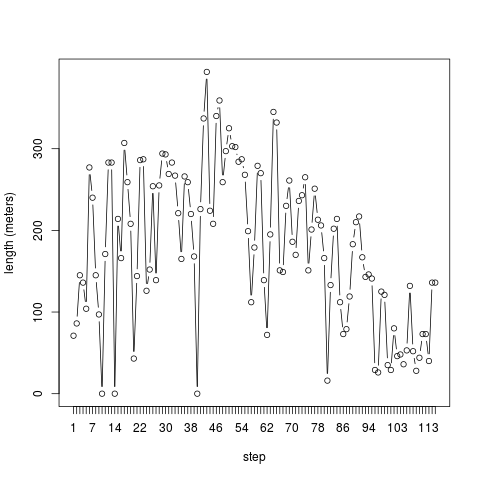
\includegraphics[width=\linewidth]{test_100_1}
  \caption*{Toàn bộ di chuyển chuyến xe 1 - đúng giờ}
\endminipage
\minipage{0.25\textwidth}
  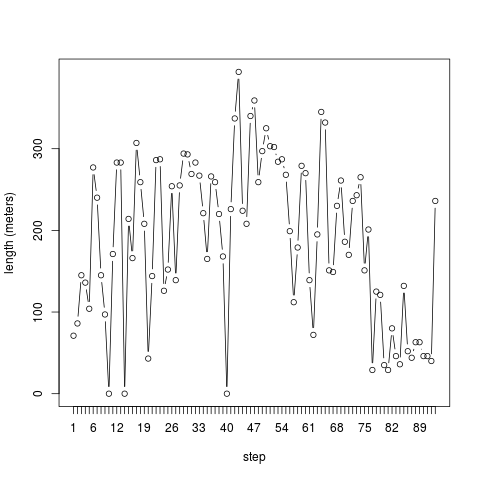
\includegraphics[width=\linewidth]{test_80_1}
  \caption*{80\% di chuyển chuyến xe 1 - đúng giờ}
\endminipage
\minipage{0.25\textwidth}%
  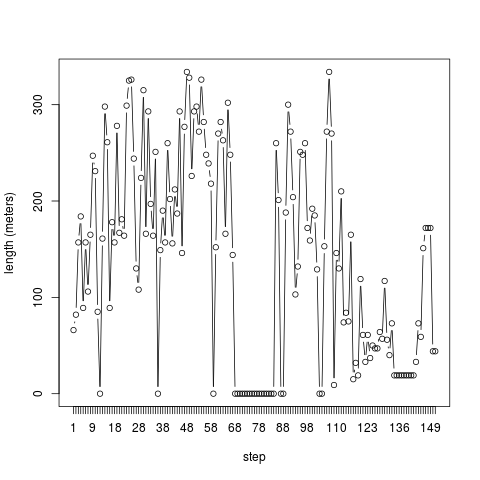
\includegraphics[width=\linewidth]{test_100_2}
  \caption*{Toàn bộ di chuyển chuyến xe 2 - trễ giờ}
\endminipage
\minipage{0.25\textwidth}
  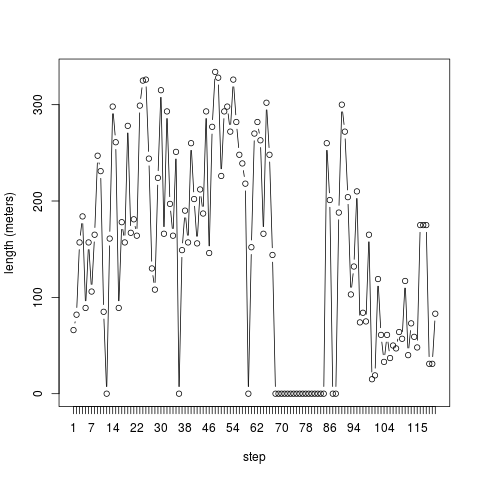
\includegraphics[width=\linewidth]{test_80_2}
  \caption*{80\% di chuyển chuyến xe 2 - trễ giờ}
\endminipage\\
\minipage{0.25\textwidth}
  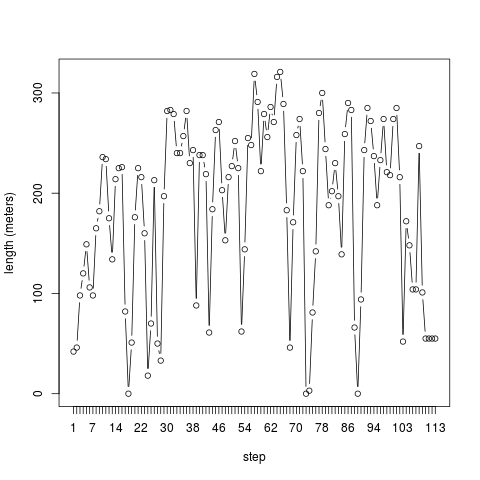
\includegraphics[width=\linewidth]{test_100_3}
  \caption*{Toàn bộ di chuyển chuyến xe 3 - đúng giờ}
\endminipage
\minipage{0.25\textwidth}
  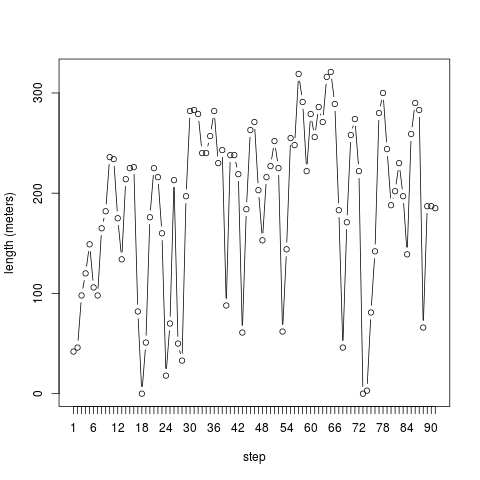
\includegraphics[width=\linewidth]{test_80_3}
  \caption*{80\% di chuyển chuyến xe 3 - đúng giờ}
\endminipage
\minipage{0.25\textwidth}%
  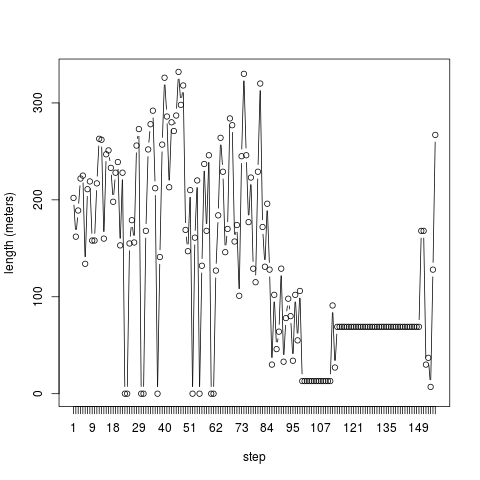
\includegraphics[width=\linewidth]{test_100_4}
  \caption*{Toàn bộ di chuyển chuyến xe 4 - trễ giờ}
\endminipage
\minipage{0.25\textwidth}
  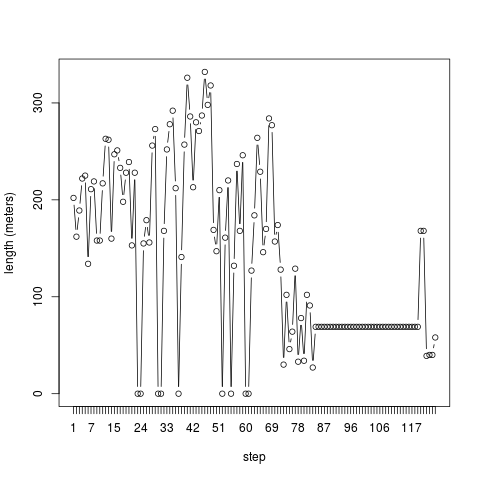
\includegraphics[width=\linewidth]{test_80_4}
  \caption*{80\% di chuyển chuyến xe 4 - trễ giờ}
\endminipage\\
\minipage{0.25\textwidth}
  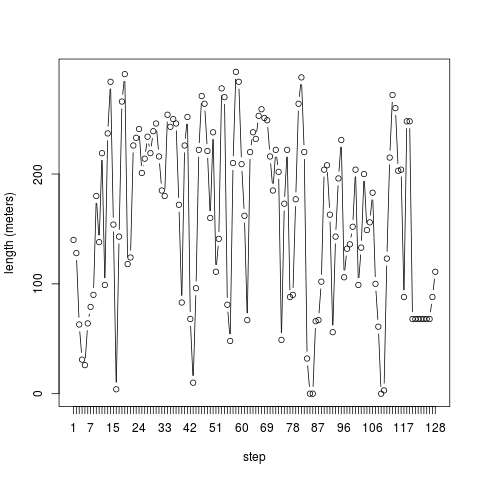
\includegraphics[width=\linewidth]{test_100_5}
  \caption*{Toàn bộ di chuyển chuyến xe 5 - đúng giờ}
\endminipage
\minipage{0.25\textwidth}
  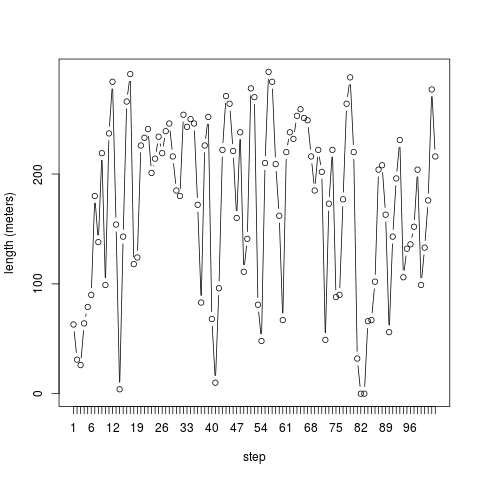
\includegraphics[width=\linewidth]{test_80_5}
  \caption*{80\% di chuyển chuyến xe 5 - đúng giờ}
\endminipage
\minipage{0.25\textwidth}%
  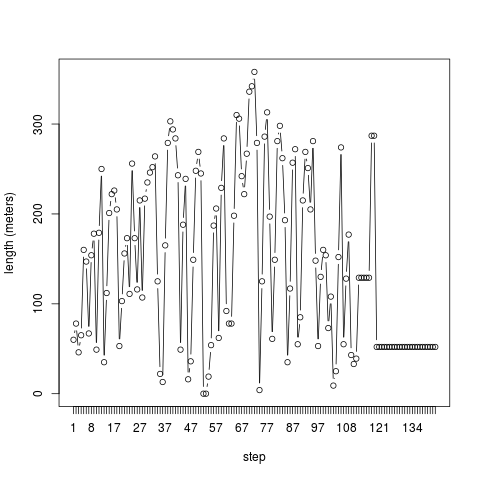
\includegraphics[width=\linewidth]{test_100_6}
  \caption*{Toàn bộ di chuyển chuyến xe 6 - trễ giờ}
\endminipage
\minipage{0.25\textwidth}
  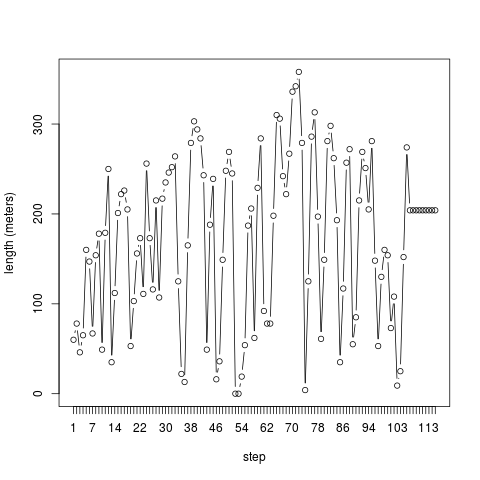
\includegraphics[width=\linewidth]{test_80_6}
  \caption*{80\% di chuyển chuyến xe 6 - trễ giờ}
\endminipage\\
\minipage{0.25\textwidth}
  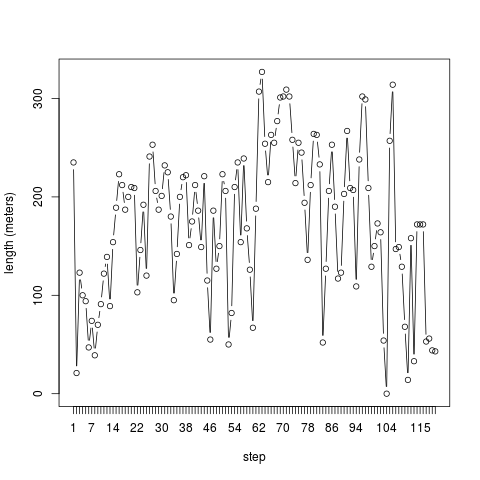
\includegraphics[width=\linewidth]{test_100_7}
  \caption*{Toàn bộ di chuyển chuyến xe 7 - đúng giờ}
\endminipage
\minipage{0.25\textwidth}
  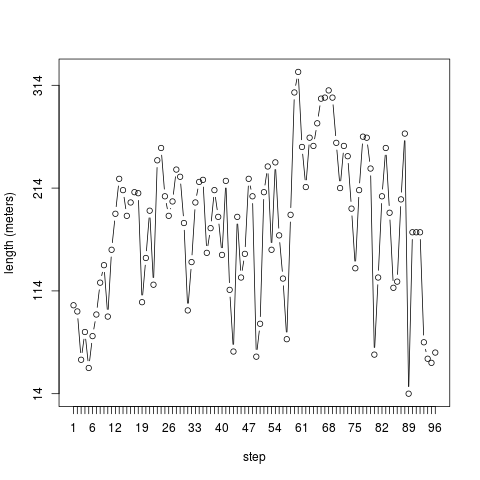
\includegraphics[width=\linewidth]{test_80_7}
  \caption*{80\% di chuyển chuyến xe 7 - đúng giờ}
\endminipage
\minipage{0.25\textwidth}%
  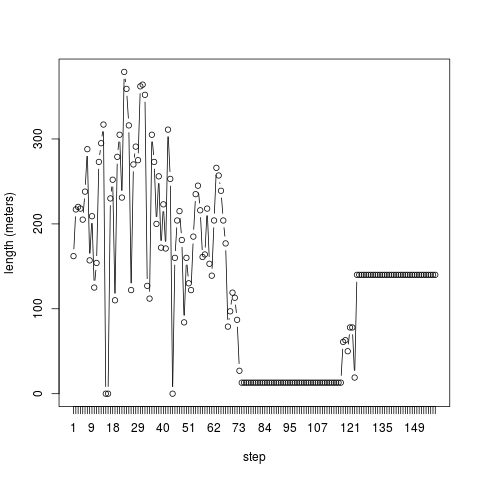
\includegraphics[width=\linewidth]{test_100_8}
  \caption*{Toàn bộ di chuyển chuyến xe 8 - trễ giờ}
\endminipage
\minipage{0.25\textwidth}
  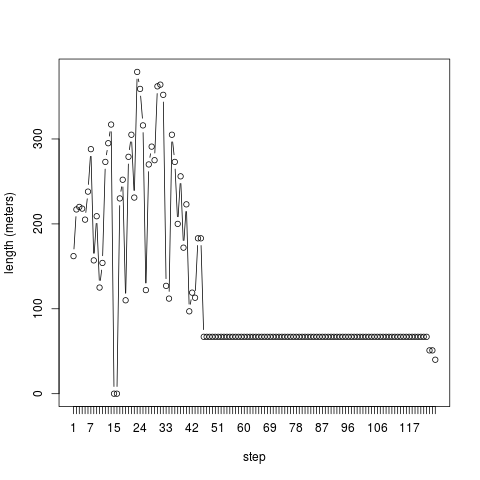
\includegraphics[width=\linewidth]{test_80_8}
  \caption*{80\% di chuyển chuyến xe 8 - trễ giờ}
\endminipage\\
\minipage{0.25\textwidth}
  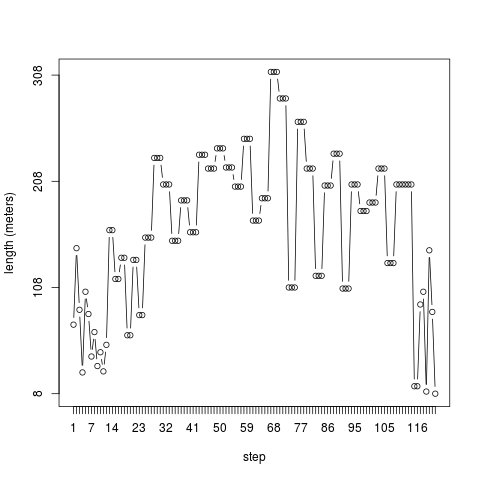
\includegraphics[width=\linewidth]{test_100_9}
  \caption*{Toàn bộ di chuyển chuyến xe 9 - đúng giờ}
\endminipage
\minipage{0.25\textwidth}
  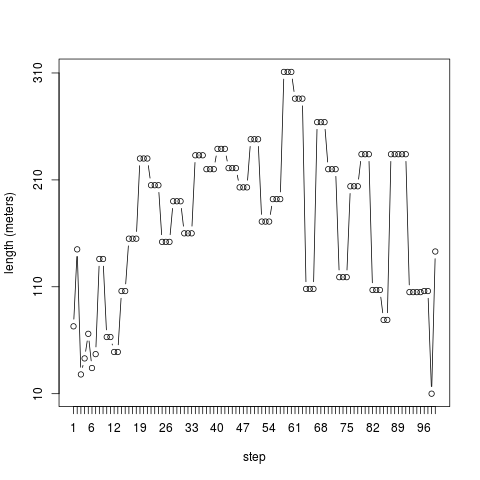
\includegraphics[width=\linewidth]{test_80_9}
  \caption*{80\% di chuyển chuyến xe 9 - đúng giờ}
\endminipage
\minipage{0.25\textwidth}%
  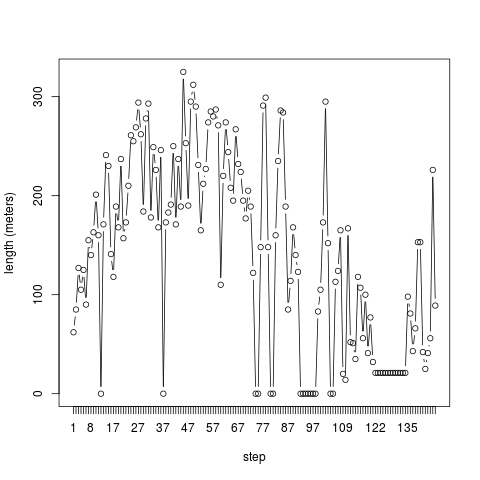
\includegraphics[width=\linewidth]{test_100_10}
  \caption*{Toàn bộ di chuyển chuyến xe 10 - trễ giờ}
\endminipage
\minipage{0.25\textwidth}
  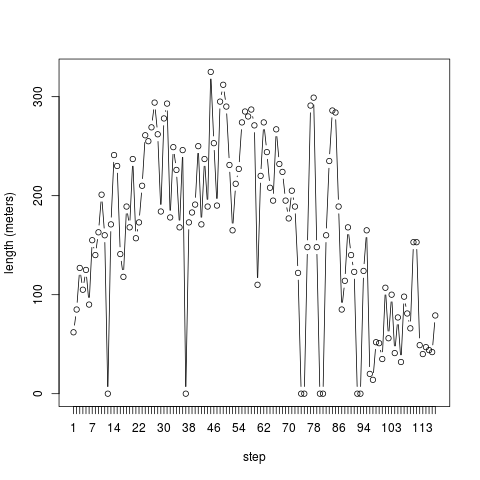
\includegraphics[width=\linewidth]{test_80_10}
  \caption*{80\% di chuyển chuyến xe 10 - trễ giờ}
\endminipage\\
\end{figure}
\FloatBarrier
\FloatBarrier
\begin{figure}[!htb]
\minipage{0.25\textwidth}
  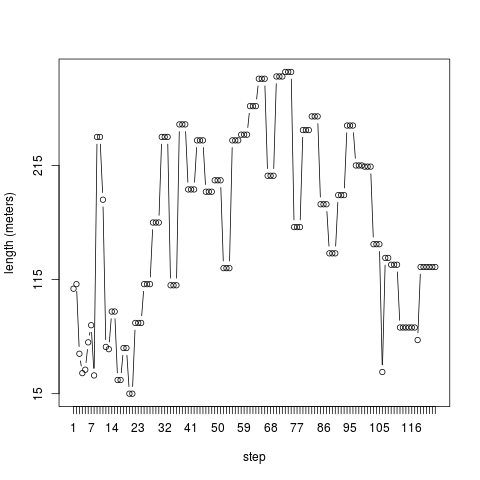
\includegraphics[width=\linewidth]{test_100_11}
  \caption*{Toàn bộ di chuyển chuyến xe 11 - đúng giờ}
\endminipage
\minipage{0.25\textwidth}
  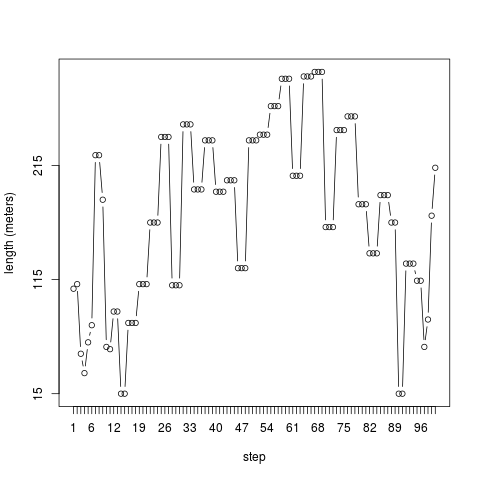
\includegraphics[width=\linewidth]{test_80_11}
  \caption*{80\% di chuyển chuyến xe 11 - đúng giờ}
\endminipage
\minipage{0.25\textwidth}%
  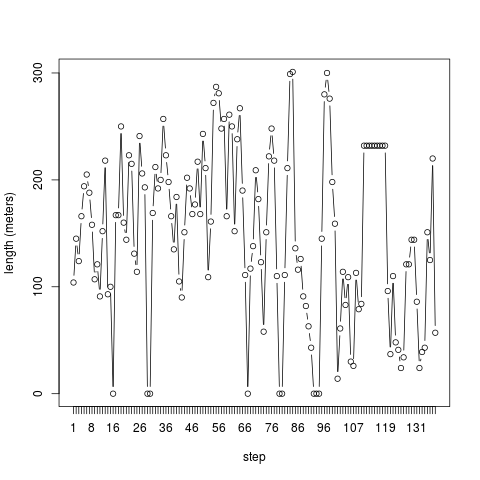
\includegraphics[width=\linewidth]{test_100_12}
  \caption*{Toàn bộ di chuyển chuyến xe 12 - trễ giờ}
\endminipage
\minipage{0.25\textwidth}
  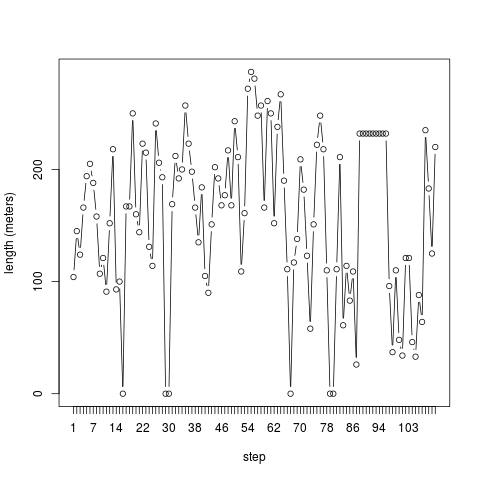
\includegraphics[width=\linewidth]{test_80_12}
  \caption*{80\% di chuyển chuyến xe 12 - trễ giờ}
\endminipage\\
\minipage{0.25\textwidth}
  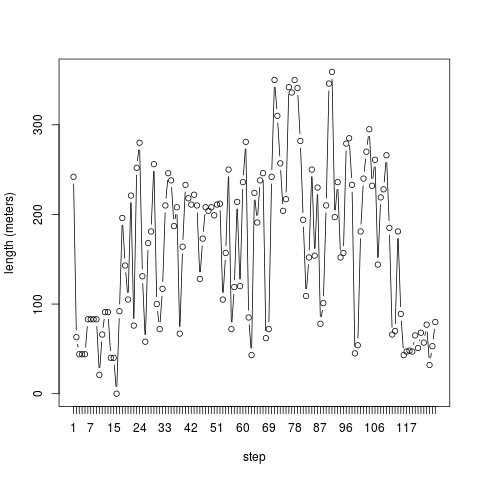
\includegraphics[width=\linewidth]{test_100_13}
  \caption*{Toàn bộ di chuyển chuyến xe 13 - đúng giờ}
\endminipage
\minipage{0.25\textwidth}
  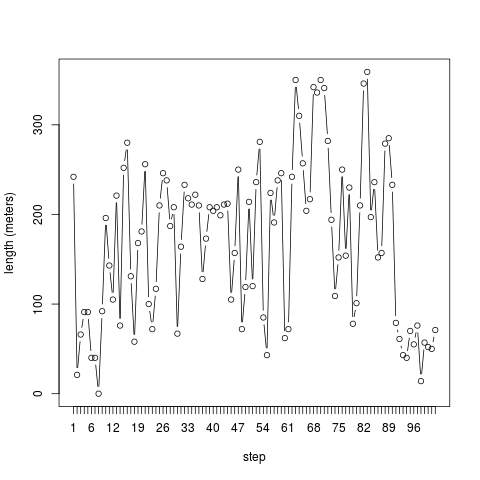
\includegraphics[width=\linewidth]{test_80_13}
  \caption*{80\% di chuyển chuyến xe 13 - đúng giờ}
\endminipage
\minipage{0.25\textwidth}%
  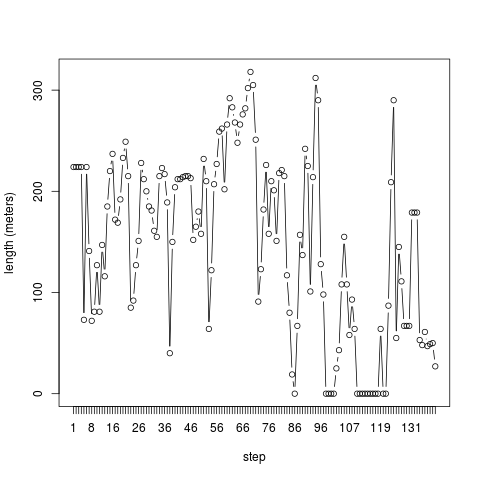
\includegraphics[width=\linewidth]{test_100_14}
  \caption*{Toàn bộ di chuyển chuyến xe 14 - trễ giờ}
\endminipage
\minipage{0.25\textwidth}
  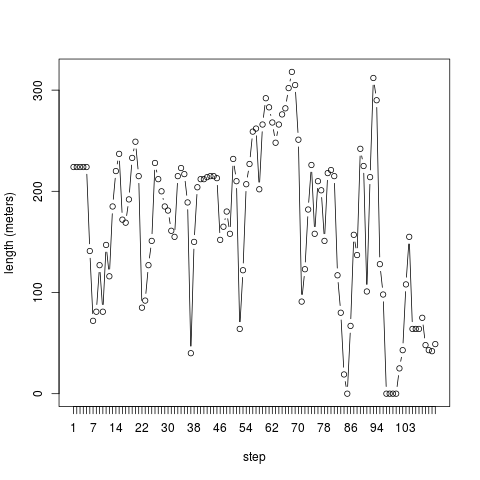
\includegraphics[width=\linewidth]{test_80_14}
  \caption*{80\% di chuyển chuyến xe 14 - trễ giờ}
\endminipage\\
\minipage{0.25\textwidth}
  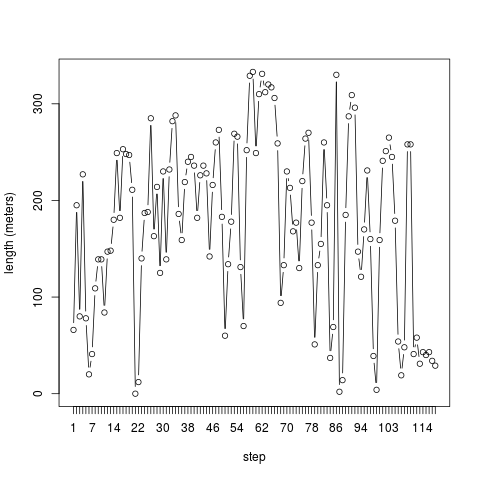
\includegraphics[width=\linewidth]{test_100_15}
  \caption*{Toàn bộ di chuyển chuyến xe 15 - đúng giờ}
\endminipage
\minipage{0.25\textwidth}
  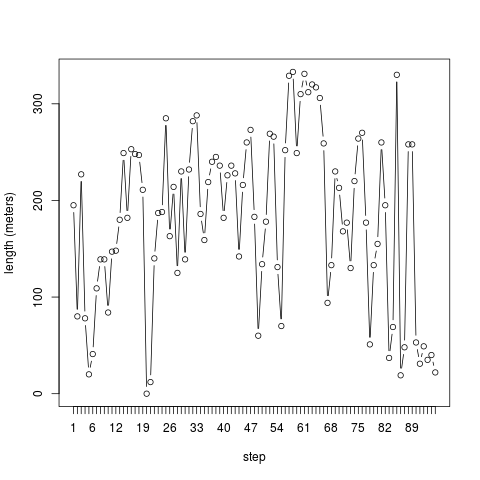
\includegraphics[width=\linewidth]{test_80_15}
  \caption*{80\% di chuyển chuyến xe 15 - đúng giờ}
\endminipage
\minipage{0.25\textwidth}%
  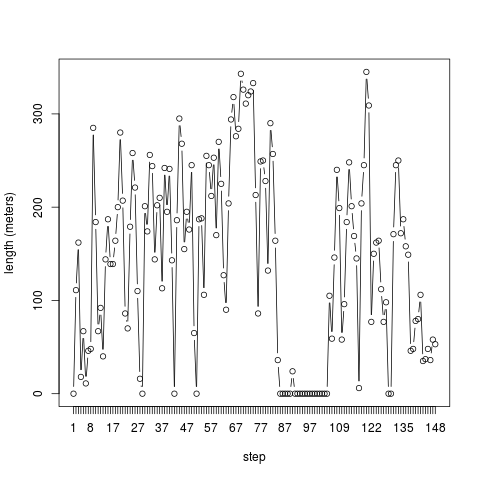
\includegraphics[width=\linewidth]{test_100_16}
  \caption*{Toàn bộ di chuyển chuyến xe 16 - trễ giờ}
\endminipage
\minipage{0.25\textwidth}
  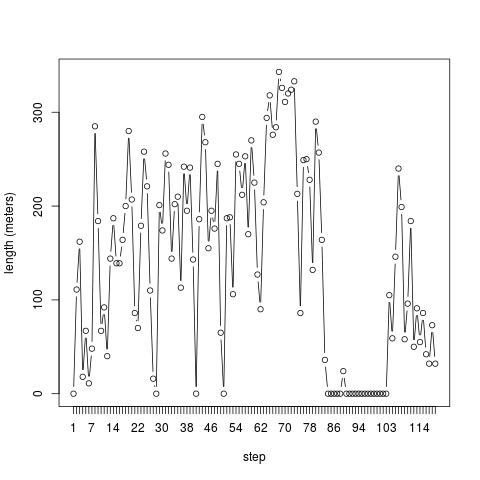
\includegraphics[width=\linewidth]{test_80_16}
  \caption*{80\% di chuyển chuyến xe 16 - trễ giờ}
\endminipage\\
\minipage{0.25\textwidth}
  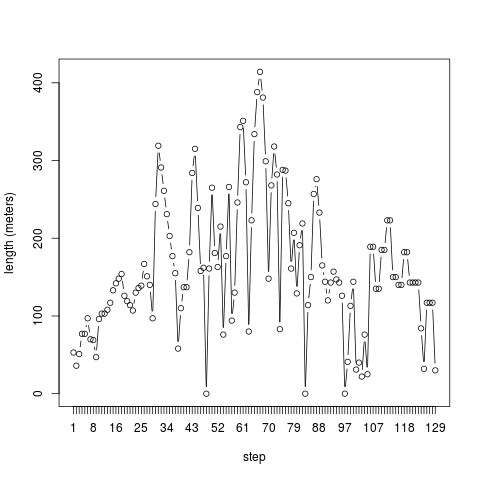
\includegraphics[width=\linewidth]{test_100_17}
  \caption*{Toàn bộ di chuyển chuyến xe 17 - đúng giờ}
\endminipage
\minipage{0.25\textwidth}
  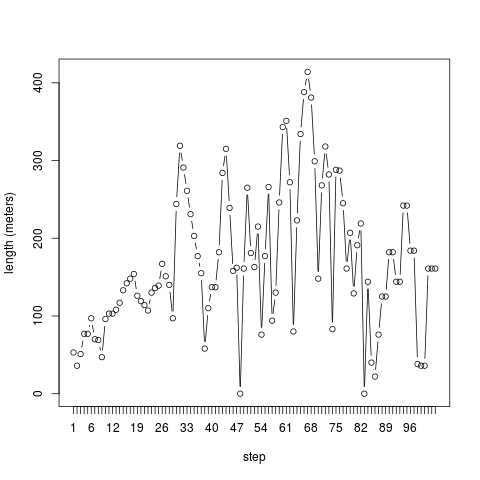
\includegraphics[width=\linewidth]{test_80_17}
  \caption*{80\% di chuyển chuyến xe 17 - đúng giờ}
\endminipage
\minipage{0.25\textwidth}%
  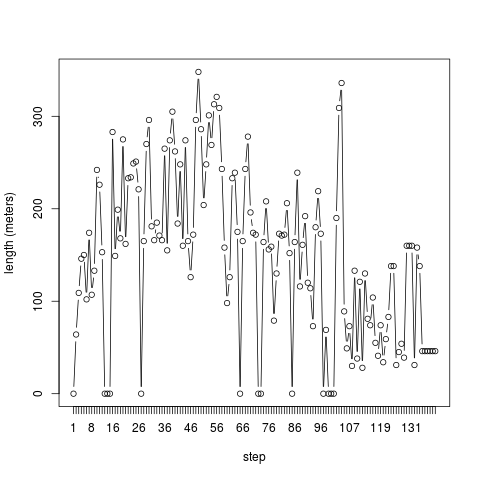
\includegraphics[width=\linewidth]{test_100_18}
  \caption*{Toàn bộ di chuyển chuyến xe 18 - trễ giờ}
\endminipage
\minipage{0.25\textwidth}
  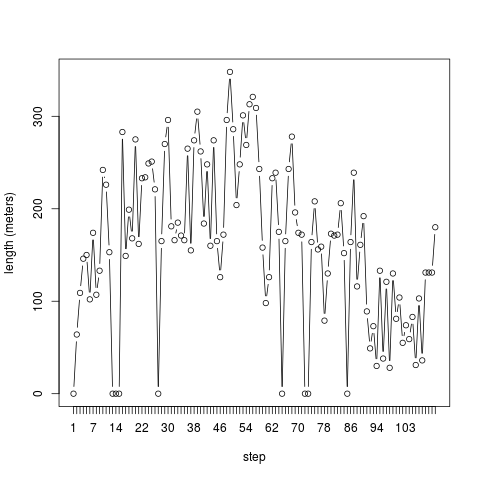
\includegraphics[width=\linewidth]{test_80_18}
  \caption*{80\% di chuyển chuyến xe 18 - trễ giờ}
\endminipage\\
\minipage{0.25\textwidth}
  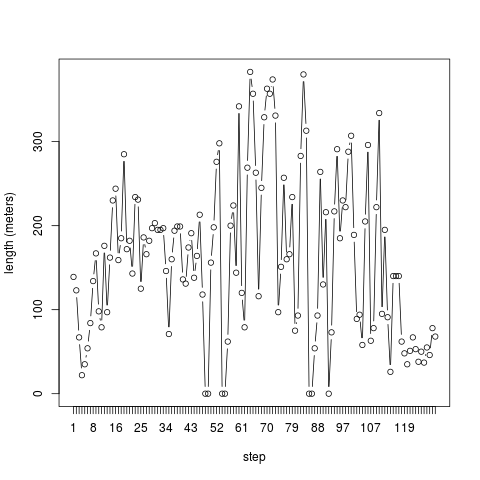
\includegraphics[width=\linewidth]{test_100_19}
  \caption*{Toàn bộ di chuyển chuyến xe 19 - đúng giờ}
\endminipage
\minipage{0.25\textwidth}
  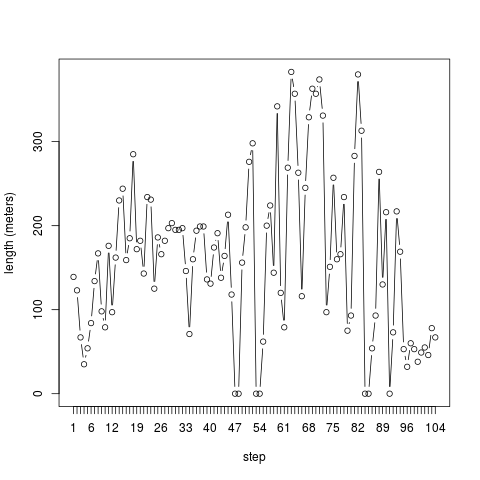
\includegraphics[width=\linewidth]{test_80_19}
  \caption*{80\% di chuyển chuyến xe 19 - đúng giờ}
\endminipage
\minipage{0.25\textwidth}%
  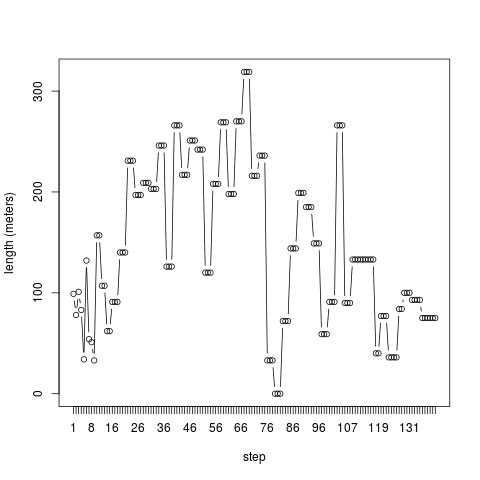
\includegraphics[width=\linewidth]{test_100_20}
  \caption*{Toàn bộ di chuyển chuyến xe 20 - trễ giờ}
\endminipage
\minipage{0.25\textwidth}
  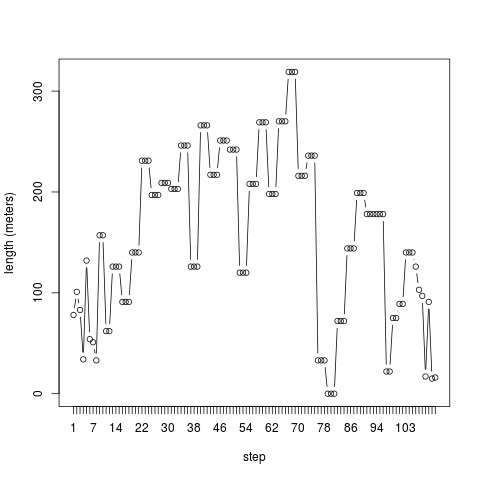
\includegraphics[width=\linewidth]{test_80_20}
  \caption*{80\% di chuyển chuyến xe 20 - trễ giờ}
\endminipage\\
\caption*{Trực quan hóa 20 dòng dữ liệu ngẫu nhiên}
\end{figure}
\FloatBarrier

Kham khảo \ref{sapxepTGHT} tại mục Phụ Lục xuất ra hình vẽ sắp xếp thời gian hoàn thành lộ trình BX Củ Chi - BX An Sương xác suất xuất hiện tăng dần.\\
\FloatBarrier
\begin{figure}[h!]
        \begin{subfigure}[b]{0.5\textwidth}
                \label{tab:example}
                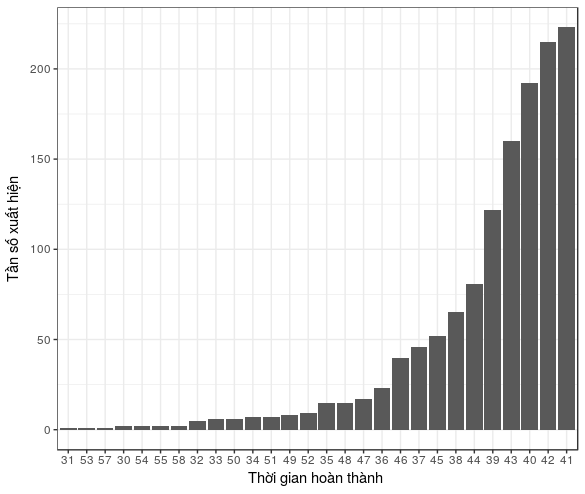
\includegraphics[width=\linewidth]{finishTime_CC_AS_Order}
        \end{subfigure}%
\end{figure}
\FloatBarrier
Kham khảo \ref{xacsuatTLTGHT} tại mục Phụ Lục xuất ra hình vẽ cho thấy xác suất tích lũy thời gian hoàn thành lộ trình BX Củ Chi - BX An Sương \\
\FloatBarrier
\begin{figure}[h!]
        \begin{subfigure}[b]{0.7\textwidth}
        		\label{tab:example2}
                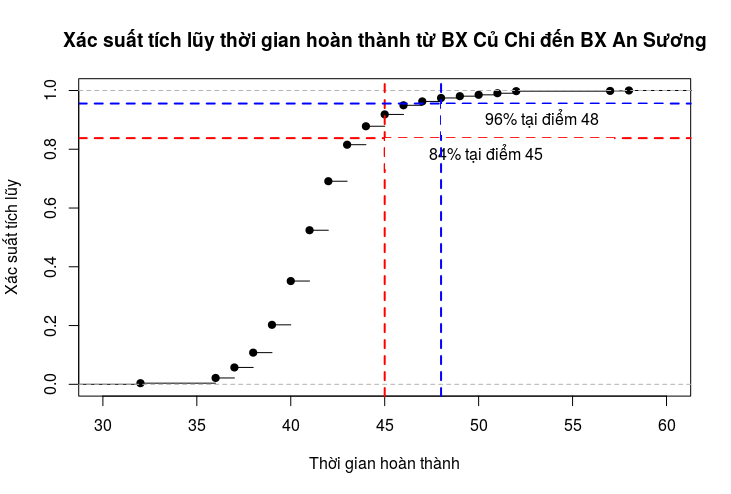
\includegraphics[width=\linewidth]{finishTime_CC_AS_ACC_Line}
        \end{subfigure}%
\end{figure}
\FloatBarrier
\section{Thu thập thông tin rút ra từ dữ liệu lịch sử}
Theo bài toán đặt ra, ta sẽ lấy thông tin dữ liệu 2/3 chuyến và phân loại thời gian đến trạm đích: đúng giờ và trễ.
\section{Tiến hành dự đoán xác suất xe buýt về trạm đúng thời gian}
\section{Kết luận}
\chapter{KẾT LUẬN}
\section{Tổng kết}
\section{Đóng góp của đề tài}
Vì các giá trị xác suất ... được tính trên mẫu và Luận Văn này chưa chứng minh được các xác suất đấy có thể đúng trên tổng thể với xác suất xảy ra cao, cho nên kết quả của Luận Văn này không sử dụng được trên thực tế. Nhưng đóng góp của Luận Văn này là tìm được một trong nhiều phương pháp giải có thể cho câu hỏi "Dự báo xác suất xe về trạm đúng giờ khi xe đã đi được một 2/3 khoảng đường"
\section{Hướng phát triển}
Để giải quyết bài toán của Luận Văn này triệt để hơn có hai cách tiếp cận:
\begin{itemize}
\item Cách 1: Giải bài toán này với dữ liệu cực lớn để tìm gần chính xác các xác suất .....Khi đó, tôi dự đoán sẽ nảy sinh thêm bài toán mới, xử lý các vấn đề khi làm việc trên dữ liệu cực lớn.
\item Cách 2: Vẫn xử lý trên dữ liệu mẫu nhỏ hơn rất nhiều so với tổng thể, người giải phải học thêm kiến thức Toán Thống Kê như các phương pháp thiết kế thí nghiệm, xác định phương pháp lấy mẫu chấp nhận được, phương pháp kiểm định giả thuyết, ..., để đủ tự tin chứng minh rằng kết quả thu được từ mẫu cũng phản ánh đúng trên tổng thể với xác suất xảy ra cao.
\end{itemize}
\pagebreak
\chapter{PHỤ LỤC}
\begin{enumerate}[label=\textbf{PL\arabic*}]
\item Mã nguồn R chạy giải thuật Jenks Natural breaks optimization
\begin{flushleft}
\begin{tabular}{  |l| }
\hline 
\textit{\#set your working directory where your file data locates}\\
setwd("/home/thuy/workspace/Preprocess")\\
mydata = read.csv("freqVeryHigh.csv")[,1]\\
mydata\\
\textit{\#returned result}\\
\textit{\# [1]  0  1  2  3  4  5  6  7  8  9 10 11}\\
\textit{\#use library classInt to run algorithm Jenks Natural breaks optimization}\\
library("classInt")\\
classIntervals(mydata, n=5, style="jenks")\\
\textit{\#returned result}\\
\textit{\#[0,1]  (1,3]  (3,5]  (5,8] (8,11]}\\
\textit{\#2      2      2      3      3 }\\
\textit{\#or use library BAMMtools to run algorithm Jenks Natural breaks optimization}\\
library("BAMMtools")\\
getJenksBreaks(mydata, 5)\\
\textit{\#returned result}\\
\textit{\#0  2  5  8 11}\\
\hline
\end{tabular}
\end{flushleft}
\item  \label{trucquandichuyen} Mã nguồn R trực quan hóa giá trị các bước di chuyển của 24 chuyến xe trên\\
\begin{flushleft}
\begin{tabular}{ |l| }
\hline 
\textit{\#set your working directory where your file data locates}\\
setwd("/home/thuy/workspace/Preprocess")\\
\textit{\#count maximum column length}\\
count.fields("data.txt", sep = ",")\\
maxCol <- max(count.fields("data.txt", sep = ","))\\
\textit{\#load data with different column length}\\
dat=read.table("data.txt", header = FALSE, \\
\hspace{2cm} col.names = 1:maxCol, \textit{\#maxCol is maximum column length in your data row}\\ 				
\hspace{2cm} sep = ",",\\ 
\hspace{2cm} fill = TRUE) \textit{\#set value NA for empty column}\\
i=1\\
for (i in 1:nrow(dat)) \{ \\
  \hspace{1cm} d=dat[i,] \textit{\# get row data}\\
  \hspace{1cm} d=d[!is.na(d)] \textit{\#remove column NA}\\
  \hspace{1cm} x=length(d)\\
  \hspace{1cm} \textit{\#capture image}\\
  \hspace{1cm} png(filename=paste("capture", i, ".png", sep = ""))\\
  \hspace{1cm} \textit{\#remove axes}\\
  \hspace{1cm} temp <- plot(1:x, d, type='b', axes=FALSE, xlab = "step", ylab = "length (meters)")\\
  \hspace{1cm} \textit{\#adjust axes length}\\  
  \hspace{1cm} temp <- axis(side=1, at=c(1:x))\\
  \hspace{1cm} temp <- axis(side=2, at=seq(min(d), max(d), by=100))\\
  \hspace{1cm} temp <- box()\\
  \hspace{1cm} print(temp)\\
  \hspace{1cm} dev.off()\\
  \}
\\
\hline
\end{tabular}
\end{flushleft}
\item \label{xacsuatTLTGHT} Mã nguồn R xuất hình thể hiện xác suất tích lũy thời gian hoàn thành BX Củ Chi - BX An Sương\\
\begin{flushleft}
\begin{tabular}{ |l| }
\hline
\textit{\#set your working directory where your file data locates}\\
setwd("/home/thuy/workspace/Preprocess")\\
y = read.csv("CC\_AS\_Rep.csv",header=FALSE)\$V1\\
p = ecdf(y)\\
plot(p,\\
\hspace{1cm} xlab = 'Thời gian hoàn thành', \\
\hspace{1cm} ylab = 'Xác suất tích lũy', \\
\hspace{1cm} main = 'Xác suất tích lũy thời gian hoàn thành từ BX Củ Chi đến BX An Sương'
)\\
abline(v = 45, h = 0.83773583,col="red",lwd=2, lty=2)\\
legend(45, 0.83773583, '84\% tại điểm 45', box.lwd = 0)\\
abline(v = 48, h = 0.9554717,col="blue",lwd=2, lty=2)\\
legend(48, 0.9554717, '96\% tại điểm 48', box.lwd = 0)\\ 
\hline
\end{tabular}
\end{flushleft}
\item \label{sapxepTGHT} Mã nguồn R sắp xếp tăng dần xác suất thời gian hoàn thành BX Củ Chi - BX An Sương\\
\begin{flushleft}
\begin{tabular}{ |l| }
\hline
\textit{\#set your working directory where your file data locates}\\
setwd("/home/thuy1/git/predictUsingProbability/Preprocess/")\\
mydata = read.csv("CC\_AS\_Freq.csv",sep = "|",header=FALSE)[ ,1:2]\\
\textit{\#set column name for your data}\\
colnames(mydata) <- c("X1","X2")\\
X1=mydata\$X1\\
X2=mydata\$X2\\
mydata\$X1 <- factor(mydata\$X1, levels = mydata\$X1[order(mydata\$X2)])\\
library(ggplot2)\\
ggplot(mydata, aes(x = mydata\$X1, y = mydata\$X2)) +\\
\hspace{1cm} theme\_bw() + geom\_bar(stat = "identity") + \\
\hspace{1cm} xlab("Thời gian hoàn thành ") +\\
\hspace{1cm} ylab("Tần số xuất hiện") \\
\hline
\end{tabular}
\end{flushleft}
\item \label{DragAndDrop} Ứng dụng bản demo "Drag And Drop data layer GeoJSON" \footnote{https://developers.google.com/maps/documentation/javascript/examples/layer-data-dragndrop} của Google Map API để kiểm tra lộ trình\\
\FloatBarrier
\begin{figure}[h]
\caption{Ứng dụng bản demo "Drag And Drop data layer GeoJSON"}
    \begin{subfigure}[b]{0.4\textwidth}
        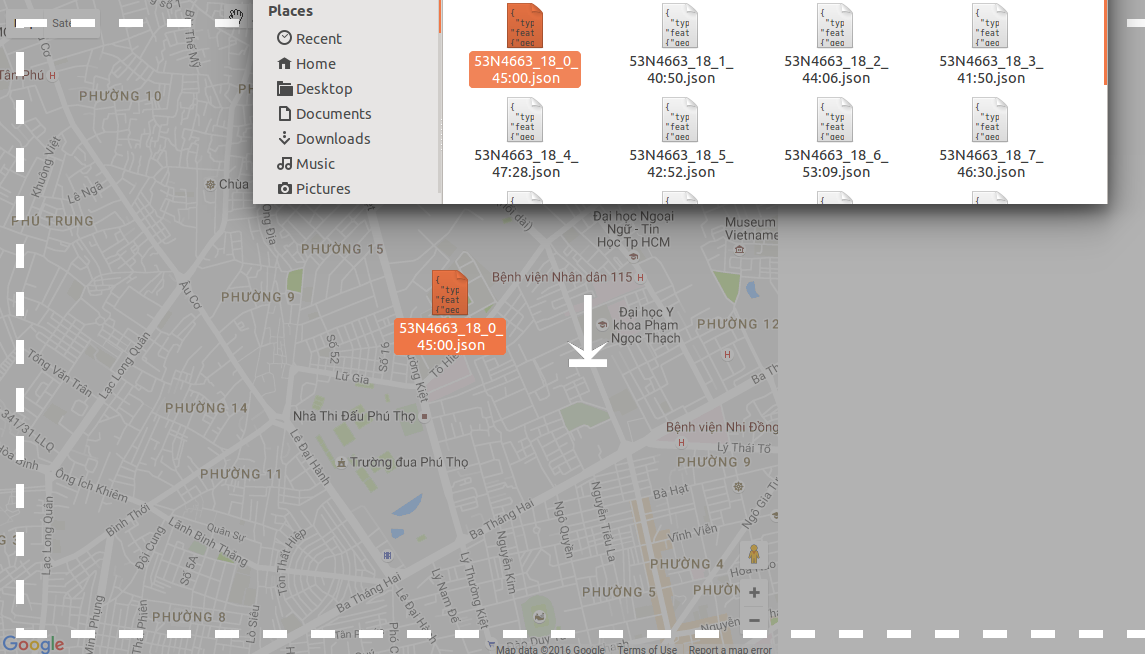
\includegraphics[width=\textwidth]{dragAndDrop1.png}
        \caption{Thả file có định dạng lớp dữ liệu GeoJSon vào bản đồ}
    \end{subfigure}
    \begin{subfigure}[b]{0.4\textwidth}
        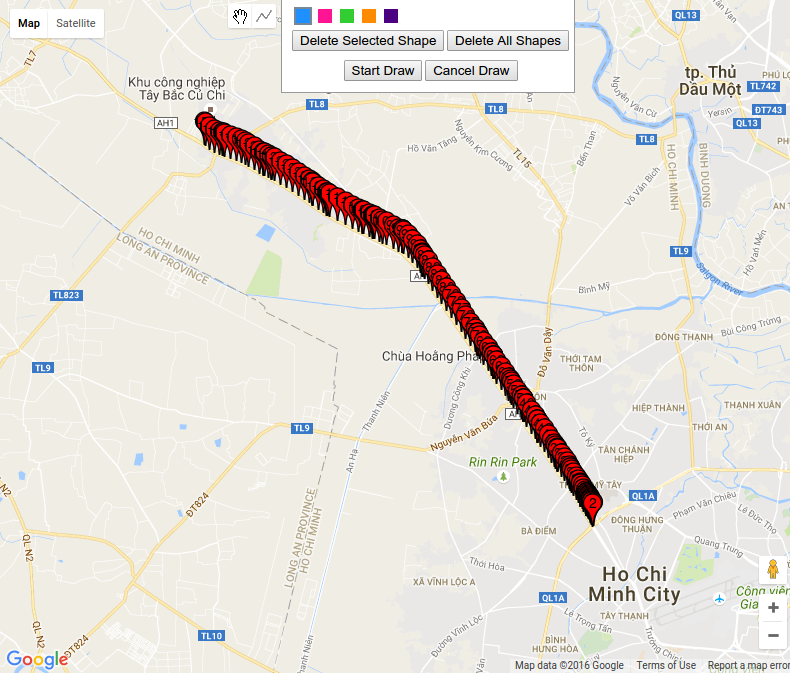
\includegraphics[width=\textwidth]{dragAndDrop2.png}
        \caption{Lớp dữ liệu GeoJson vừa thả xuất hiện trên bản đồ}
    \end{subfigure}
\end{figure}
\FloatBarrier

\item \label{tinhkhoangcach} Mã nguồn Java tính khoảng cách giữa 2 tọa độ
\begin{flushleft}
\begin{tabular}{ |l| }
\hline
public static float distFrom(double lat1, double lng1, double lat2, double lng2) \{\\
\hspace{0.5cm} double earthRadius = 6371000; //meters\\
\hspace{0.5cm} double dLat = Math.toRadians(lat2-lat1);\\
\hspace{0.5cm} double dLng = Math.toRadians(lng2-lng1);\\
\hspace{0.5cm} double a = Math.sin(dLat/2) * Math.sin(dLat/2) +\\
\hspace{2.3cm} Math.cos(Math.toRadians(lat1)) * Math.cos(Math.toRadians(lat2)) *\\
\hspace{2.3cm} Math.sin(dLng/2) * Math.sin(dLng/2);\\
\hspace{0.5cm} double c = 2 * Math.atan2(Math.sqrt(a), Math.sqrt(1-a));\\
\hspace{0.5cm} float dist = (float) (earthRadius * c);\\
\hspace{0.5cm} return dist;\\
\}\\
\hline
\end{tabular}
\end{flushleft}

\item \label{dongbohoa20} Mã nguồn Java tính gom nhóm theo chuẩn 20 giây 
\begin{flushleft}
\begin{tabular}{ |l| }
\hline
function filterStandardResponse(List<Long> responseDurationList) \{\\
\hspace{0.5cm} List<Long> nonStandardList = new ArrayList<Long>();\\
\hspace{0.5cm} for (Long duration: responseDurationList) \{\\
\hspace{1cm} if (duration \% 20 == 0) \{\\
\hspace{1.5cm} break2StandardResponse(duration);\\
\hspace{1cm} \} else \{\\
\hspace{1.5cm} nonStandardList.add(duration); \\
\hspace{1cm} \}\\
\hspace{0.5cm} \}\\
\hspace{0.5cm} sort(nonStandardList);\\
\hspace{0.5cm} accumulate2ElmntToStandardResponse();\\
\}\\
\hline
\end{tabular}
\end{flushleft}
\begin{flushleft}
\begin{tabular}{ |l| }
\hline
function accumulate2ElmntToStandardResponse(List<Long> sortedNonStandardDurationList) \{\\
\hspace{0.5cm} List<Long> blockIndexList = new ArrayList<Long>();\\
\hspace{0.5cm} int maxIndex = sortedNonStandardDurationList.size();\\
\hspace{0.5cm} for (int i = 0; i <= maxIndex - 2; i++) \{\\
\hspace{1cm}   for (int j = 0; j <= maxIndex - 1; j++) \{\\
\hspace{1.5cm} long duration1 = sortedDuration.get(i); \\
\hspace{1.5cm} long duration2 = sortedDuration.get(j);\\
\hspace{1.5cm} long sumDuration = duration1+duration2;\\
\hspace{1.5cm} if (sumDuration \% 20 == 0 \&\& !blockList.contains(i) \&\& !blockList.contains(j)) \{\\
\hspace{2cm} blockList.add(i);\\
\hspace{2cm} blockList.add(j);\\
\hspace{2cm} break2StandardResponse(duration);\\
\hspace{1.5cm} \}\\
\hspace{1cm} \}\\
\hspace{0.5cm} \}\\
\hspace{0.5cm} List<Long> newSortedNonStandardList = new ArrayList<Long>();\\
\hspace{0.5cm} for (int i = 0; i < maxIndex; i++) \{\\
\hspace{1.5cm}     if (!blockList.contains(i)) \{\\
\hspace{2cm}        newSortedNonStandardList.add(sortedNonStandardDurationList.get(i));\\
\hspace{1.5cm}     \}\\
\hspace{0.5cm} \}\\
\hspace{0.5cm} if (newSortedNonStandardList.size() >= 3) \{\\
\hspace{1.5cm}      accumulate3ElmntToStandardResponse(newSortedNonStandardList);\\
\hspace{0.5cm} \}\\
\hline
\end{tabular}
\end{flushleft}
Các hàm accumulate3ElmntToStandardResponse và accumulate4ElmntToStandardResponse tương tự như hàm accumulate2ElmntToStandardResponse để thực hiện gom nhóm 3 thành phần, 4 thành phần thành bội số 20, cuối cùng với những thành phần chưa được gom nhóm. Tiếp theo, thực hiện việc gom nhóm các thành phần liên tiếp thành bội số 20. Cuối cùng, thực hiện gom nhóm các thành phần liên tiếp sao cho chia cho 20 có số dư nhỏ nhất\\
\begin{flushleft}
\begin{tabular}{ |l| }
\hline
function accumulateSequenceElmtToStandardResponse(List<Long> sortedNonStandardDurationList) \{\\
\hspace{0.5cm} int i = 0;\\
\hspace{0.5cm} int j = 1;\\
\hspace{0.5cm} int maxIndex = sortedNonStandardDurationList.size();\\
\hspace{0.5cm} while (i<maxIndex) \{\\
\hspace{1cm}      long sumDuration = sortedDuration.get(i);\\
\hspace{1cm}      while (j < maxIndex) \{\\
\hspace{1.5cm}       sumDuration += sortedDuration.get(j);\textit{\#sum of continuous elements}\\
\hspace{1.5cm}       if (sumDuration\%20==0) \{\\
\hspace{2cm}           break2StandardResponse(sumDuration);\\
\hspace{2cm}           i=j+1;\textit{\#create new caculation with start index equal j+1}\\
\hspace{2cm}           j=i+1;\\
\hspace{2cm}           break;\\
\hspace{1.5cm}       \} else \{\\
\hspace{2cm}           j++;\textit{\#continue until sumDuration\%20 equal 0}\\
\hspace{1.5cm}        \}\\
\hspace{1cm}       \}\\
\hspace{1cm}     if (j == maxIndex) \{\\
\hspace{1.5cm}        break;\\
\hspace{1cm}     \}\\
\hspace{0.5cm} \}\\
\hspace{0.5cm} List<Long> notAccumulateElmtList = new ArrayList<Long>();\\
\hspace{0.5cm} while (i<maxIndex) \{\\
\hspace{1cm}      notAccumulateElmtList.add(sortedNonStandardDurationList.get(i));\\
\hspace{1cm}      i++;\\
\hspace{0.5cm} \}\\
\hspace{0.5cm} accumulateSequenceElmtWithMinRedundant(notAccumulateElmtList);\\
\hline
\end{tabular}
\end{flushleft}

\begin{flushleft}
\begin{tabular}{ |l| }
\hline
function accumulateSequenceElmtWithMinRedundant(List<Long> sortedNonStandardDurationList) \{\\
\hspace{0.5cm} int i = 0;\\
\hspace{0.5cm} int j = 1;\\
\hspace{0.5cm} int stopIndex = 0;\\
\hspace{0.5cm} int maxIndex = sortedNonStandardDurationList.size();\\
\hspace{0.5cm} while (i<maxIndex) \{\\
\hspace{1cm} long sumDuration = sortedNonStandardDurationList.get(i);\\
\hspace{1cm} stopIndex = i;\\
\hspace{1cm} long compareNumber = 20;\\
\hspace{1cm} if (sumDuration/20>0) \{\textit{\#if sumDuration > 20}\\
\hspace{1.5cm}   compareNumber = 20*(sumDuration/20);\\
\hspace{1cm} \}\\
\hspace{1cm} long min = Math.abs(sumDuration - compareNumber);\\
\hspace{1cm} while (j < maxIndex) \{\\
\hspace{1.5cm}   sumDuration += sortedNonStandardDurationList.get(j);\\
\hspace{1.5cm}   long currentCompareNumber = 20;\\
\hspace{1.5cm}   if (sumDuration/20>0) \{\textit{\#if sumDuration > 20}\\
\hspace{2cm}          currentCompareNumber = 20*(sumDuration/20);\\
\hspace{1.5cm}   \}\\
\hspace{1.5cm}   long currentMin = Math.abs(sumDuration - currentCompareNumber);\\
\hspace{1.5cm}   if (currentMin <= min) \{\\
\hspace{2cm}       stopIndex = j;\\
\hspace{2cm}       min = currentMin;\\
\hspace{1.5cm}    \}\\
\hspace{1.5cm}   j++;\\
\hspace{1cm} \}\\
\hspace{1cm}  if (stopIndex != i) \{\\
\hspace{1.5cm}     sumDuration = 0;\\
\hspace{1.5cm}     for (int k = i; k <= stopIndex; k++) \{\\
\hspace{2cm}         sumDuration += sortedNonStandardDurationList.get(k);\\
\hspace{1.5cm}     \}\\  
\hspace{1.5cm}     break2StandardResponse(sumDuration);  \\            
\hspace{1cm}   \}\\
\hspace{1cm}     i = stopIndex + 1;\\
\hspace{1cm}     j = i + 1;\\
\hspace{0.5cm} \}\\
\hline
\end{tabular}
\end{flushleft}


\end{enumerate}


\clearpage
\newpage
\begin{center}{\fontsize{16pt}{1}\selectfont \textbf{LÝ LỊCH TRÍCH NGANG}}\\\end{center}
\vspace*{0.1cm}Họ và tên: Lê Thị Minh Thùy \\
\vspace*{0.1cm}Ngày sinh: 22/01/1986 \\
\vspace*{0.1cm}Nơi sinh: Đồng Nai \\
\vspace*{0.1cm}Địa chỉ liên lạc: 741 Trương Công Định Phường 9, TP Vũng Tàu \\
\vspace*{0.1cm}Email: thuyltm2201@gmail.com \\
\vspace*{0.1cm}\textbf{QUÁ TRÌNH ĐÀO TẠO}\\
\vspace*{0.5cm}\begin{tabular}{ |c|c|c|c| } 
\hline
 Thời gian & Trường đào tạo & Chuyên ngành & Trình độ đào tạo\\
\hline
 2004 – 2009 & Trường Đại học Bách Khoa TP.HCM & Công nghệ thông tin & Cử nhân\\
\hline 
 2013 – 2017 & Trường Đại học Bách Khoa TP.HCM & Khoa học máy tính & Thạc sĩ\\
\hline
\end{tabular}\\
\vspace*{0.5cm}\textbf{QUÁ TRÌNH CÔNG TÁC}\\
\vspace*{0.5cm}\begin{tabular}{ |c|p{9.8cm}|c| } 
\hline
 Thời gian & Đơn vị công tác & Chuyên ngành\\
\hline
 2014 – 2016 & Công ty gia công phần mềm Tường Minh & Lập trình viên\\
\hline 
\end{tabular}

\cleardoublepage
\addcontentsline{toc}{chapter}{DANH MỤC KHAM KHẢO}
\begin{thebibliography}{9}
\section*{Tài liệu trong nước}
\bibitem{TKCNUDR}	
	Người dịch: Nguyễn Văn Minh Mẫn, 
	\emph{Thống kê Công nghiệp hiện đại với ứng dụng viết trên R, MINITAB và JMP},
	Nhà xuất bản Bách Khoa Hà Nội,2016, pp.19-131
\section*{Tài liệu nước ngoài}
\bibitem{Brockwell_intro}
	Jiawei Han, Micheline Kamber, Jian Pei (2012),
	\emph{Data Mining: Concepts and Techniques (3rd ed.)},
	Morgan Kaufmann Publishers, USA.
\section*{Website}
\bibitem{JNBO}
	\emph{Jenks natural breaks optimization}, truy cập ngày 23 tháng 10 năm 2016,
	địa chỉ \emph{https://en.wikipedia.org/wiki/Jenks\_natural\_breaks\_optimization}.\\
\bibitem{JNBOE}
	\emph{Jenks natural breaks optimization example}, truy cập ngày 18 tháng 2 năm 2017,
	địa chỉ \emph{https://www.ehdp.com/vitalnet/breaks-1.htm}.
\bibitem{2WAYSOFNB}
	\emph{2 ways of using Naive Bayes classification for numeric attributes}, truy cập ngày 1 tháng 3 năm 2017,
	địa chỉ \emph{http://www.simafore.com/blog/bid/107702/2-ways-of-using-Naive-Bayes-classification-for-numeric-attributes}..
\bibitem{Gaussian classifier}
	\emph{The Gaussian classifier}, truy cập ngày 2 tháng 3 năm 2017,
	địa chỉ \emph{http://www.svcl.ucsd.edu/courses/ece271A/handouts/GC.pdf}.
	
		
	
\section*{Developer's Website}
\bibitem{GeoJSON}
	\emph{Google Maps 3 API - Data Layer: GeoJSON}, truy cập ngày 6 tháng 11 năm 2016,
	địa chỉ \emph{https://developers.google.com/maps/documentation/javascript/examples/layer-data-style}.	
\bibitem{DADG}
	\emph{Google Maps 3 API - Click on feature (from geojson)}, truy cập ngày 6 tháng 11 năm 2016,
	địa chỉ \emph{http://stackoverflow.com/questions/29309856/google-maps-3-api-click-on-feature-from-geojson-and-check-if-it-contains-loc}.
\bibitem{DADG}
	\emph{Google Maps 3 API - Data Layer: Drag and Drop GeoJSON}, truy cập ngày 6 tháng 11 năm 2016,
	địa chỉ \emph{https://developers.google.com/maps/documentation/javascript/examples/layer-data-dragndrop}.		
\bibitem{WID}
	\emph{Google Maps 3 API - Waypoints in directions}, truy cập ngày 6 tháng 11 năm 2016,
	địa chỉ \emph{https://developers.google.com/maps/documentation/javascript/examples/directions-waypoints}.	
\bibitem{DM}
	\emph{Google Maps 3 API - Distance Matrix}, truy cập ngày 6 tháng 11 năm 2016,
	địa chỉ \emph{https://developers.google.com/maps/documentation/javascript/examples/distance-matrix}.	
\end{thebibliography}
\pagebreak
\end{document}

